%\documentclass[prb,twocolumn,showpacs,aps,floats,floatfix,superscriptaddress]{revtex4}
%\documentclass[prb,showpacs,aps,floats,floatfix,superscriptaddress]{revtex4}
%\documentclass{article}
%\documentclass[12pt]{scrreprt}
%\documentclass[onecolumn,letterpaper,amsmath,amssymb,floatfix,aps,superscriptaddress]{revtex4}
\documentclass[a4paper]{article}
\usepackage{epsfig,amsmath,amssymb,array,dcolumn,subfigure,rotating,graphicx}
%\usepackage{graphicx}% Include figure files

%\usepackage{datetime}
\title{\bf Python results Hamaker coefficients for perpendicular [6,5], [9,0],
[9,1], [9,3], and [29,0] cylinders in water using retarded and non-retarded formulations.}
\author{JC Hopkins}

\begin{document}
\maketitle
\begin{abstract}
Comparison of contributions of Matsubara sums to the retarded formulation for\\
Hamaker coeffiecient, ${\cal A}^{(0)}$.  I choose to use [6,5], a
semiiconductor,\\
and [9,3], a semimetal, as examples. All caluclations are for identical pairs
of\\
CNTs in water with a mutual angle of $\pi/2$. \\
\\
Equations correspond to those in version 4 of Rudi's report.
\end{abstract}
\tableofcontents

%%%%%%%%%EPS2 and Aiz%%%%%%%%%%%%%%%%%%%%%%%%%%%%%%%%%%%%%%%%%%%%%%%%
\section{CNTs}
%\addtocontents{toc}{This is the text we'd like to add
%to the table of contents.\par}
\subsection{[6,5] Dielectric response spectrum, dispersion spectrum, and anisotropy measure}
\begin{center}
    From the imaginary part of the dielectric response function of the carbon
nanotubes, \\we compute the London dispersion spectrum by the Kramers-Kronig
transform:
\begin{equation}
\epsilon(i \zeta_n) = 1 + \frac{\pi}{2} \int_0^{\infty} dw
~\frac{\epsilon\prime\prime(\omega)\omega}{\omega^{2} + \zeta^{2}}
\end{equation}
%Where $\zeta_n = 2\pi n k_BT/\hbar$, and $n$ is an integer and the $n=0$ term is counted with a weight $1/2$. 

Relative anisotropy measures in the parallel and perpendicular direction are given by
\begin{equation}
\Delta_{\perp}=\frac{{\epsilon^{c}}_{\perp}-\epsilon_{m}}{{\epsilon^{c}}_{\perp}+\epsilon_{m}}\qquad\Delta_{\parallel}=\frac{{\epsilon^{c}}_{\parallel}-\epsilon_{m}}{\epsilon_{m}}.
\label{anisoind}
\end{equation}

Ratio of anisotropy measure:
\begin{equation}
a_{1,2}(i \omega_n) = \frac{2 \Delta_{\perp}^{(1,2)}(i\omega_n)}{\Delta_{\parallel}^{(1,2)}(i \omega_n)} = 
2 \frac{({{\epsilon^{c}}_{\perp}}^{(1,2)}(i \omega_n) -\epsilon_{m}(i \omega_n)) \epsilon_{m}(i \omega_n)}{({{\epsilon^{c}}_{\perp}}^{(1,2)}(i \omega_n)+\epsilon_{m}(i \omega_n)) ({{\epsilon^{c}}_{\parallel}}^{(1,2)}(i \omega_n) -\epsilon_{m}(i \omega_n))}
\label{eq:adef}
\end{equation}

For interactions between identical CNTs, we set $a_{1}=a_{2}$.  

\begin{figure*}[t!]
\begin{center}
\begin{minipage}[b]{0.40\textwidth}
\begin{center}
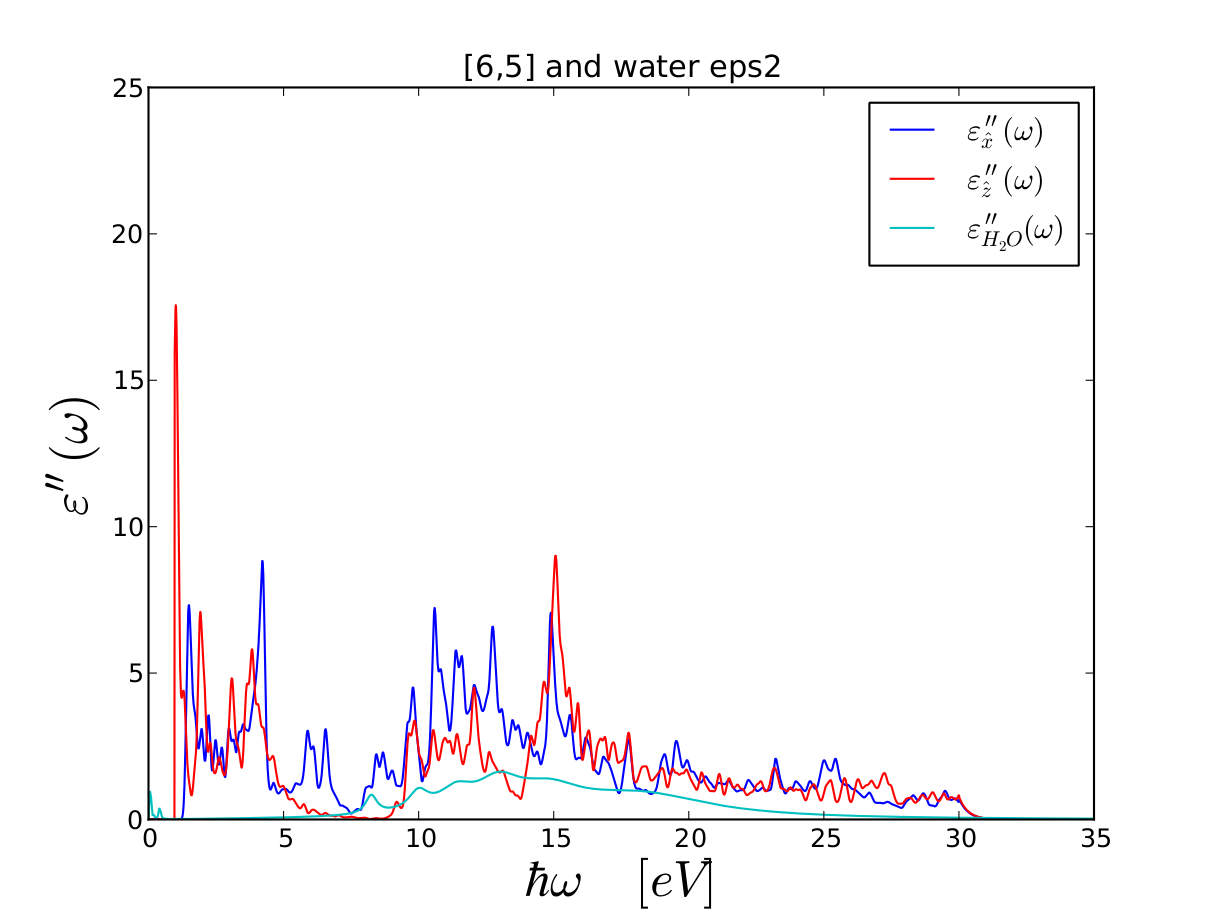
\includegraphics[width=1.4\textwidth]{prop_plots/65w65_eps2.png} (a)
\end{center}
\end{minipage}
\hskip 43pt
\begin{minipage}[b]{0.40\textwidth}
\begin{center}
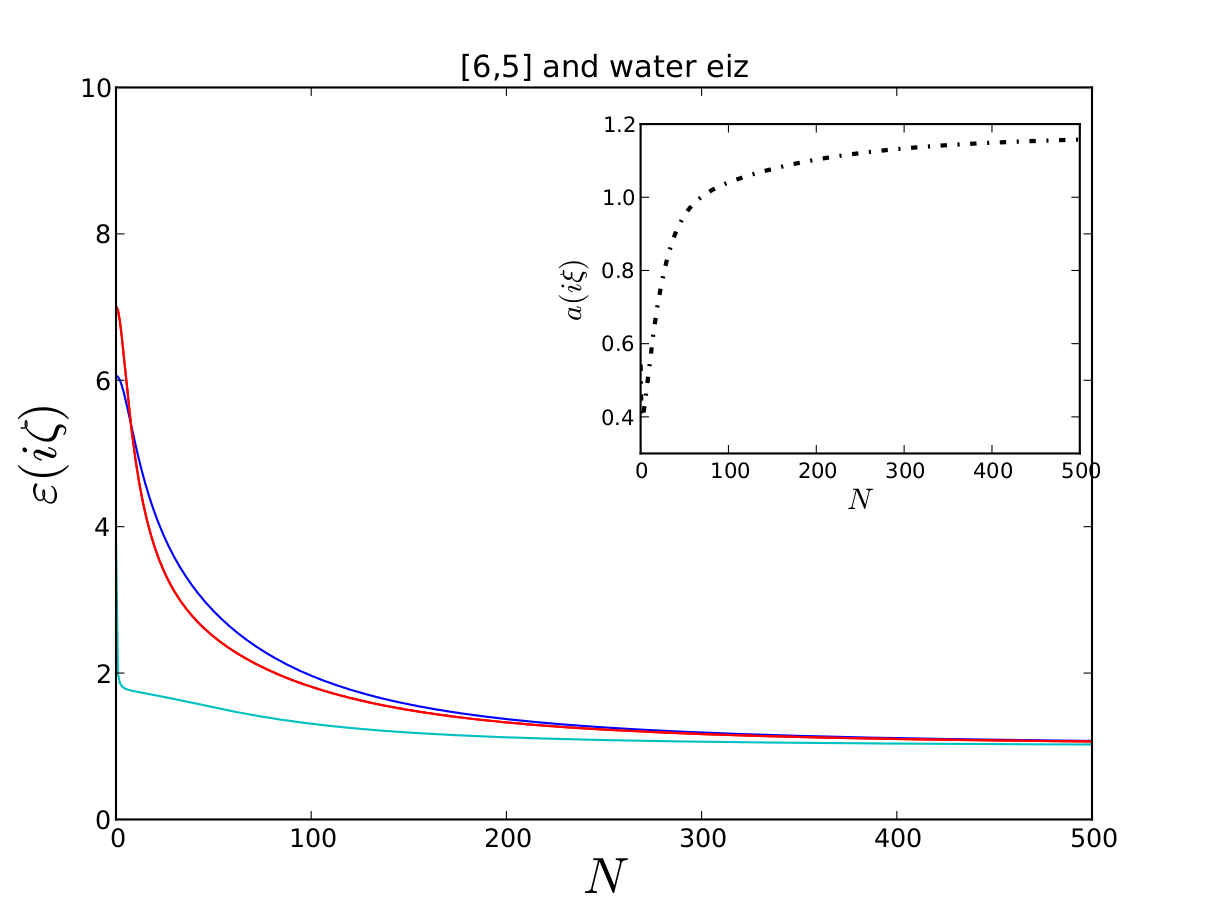
\includegraphics[width=1.4\textwidth]{prop_plots/65w65_eiz.png} (b)
\end{center}
\end{minipage}
\caption{(a) Imaginary dielectric response spectrum, (b) dispersion spectrum and anisotropy measure (inset)}
\label{eiz65}
\end{center}
\end{figure*} 

%%%%%%%%%EPS2 and Aiz%%%%%%%%%%%%%%%%%%%%%%%%%%%%%%%%%%%%%%%%%%%%%%%%
\section{[9,0] dielectric response spectrum, dispersion spectrum, and anisotropy measure}
Relative anisotropy measures in the parallel and perpendicular direction are given by
\begin{equation}
\Delta_{\perp}=\frac{{\epsilon^{c}}_{\perp}-\epsilon_{m}}{{\epsilon^{c}}_{\perp}+\epsilon_{m}}\qquad\Delta_{\parallel}=\frac{{\epsilon^{c}}_{\parallel}-\epsilon_{m}}{\epsilon_{m}}.
\label{anisoind}
\end{equation}

Ratio of anisotropy measures
\begin{equation}
a_{1,2}(i \omega_n) = \frac{2 \Delta_{\perp}^{(1,2)}(i\omega_n)}{\Delta_{\parallel}^{(1,2)}(i \omega_n)} = \\
2 \frac{({{\epsilon^{c}}_{\perp}}^{(1,2)}(i \omega_n) -\epsilon_{m}(i \omega_n)) \epsilon_{m}(i \omega_n)}{({{\epsilon^{c}}_{\perp}}^{(1,2)}(i \omega_n)+\epsilon_{m}(i \omega_n)) ({{\epsilon^{c}}_{\parallel}}^{(1,2)}(i \omega_n) -\epsilon_{m}(i \omega_n))}
    \label{eq:adef}
\end{equation}
\begin{figure*}[t!]
\begin{center}
\begin{minipage}[b]{0.40\textwidth}
\begin{center}
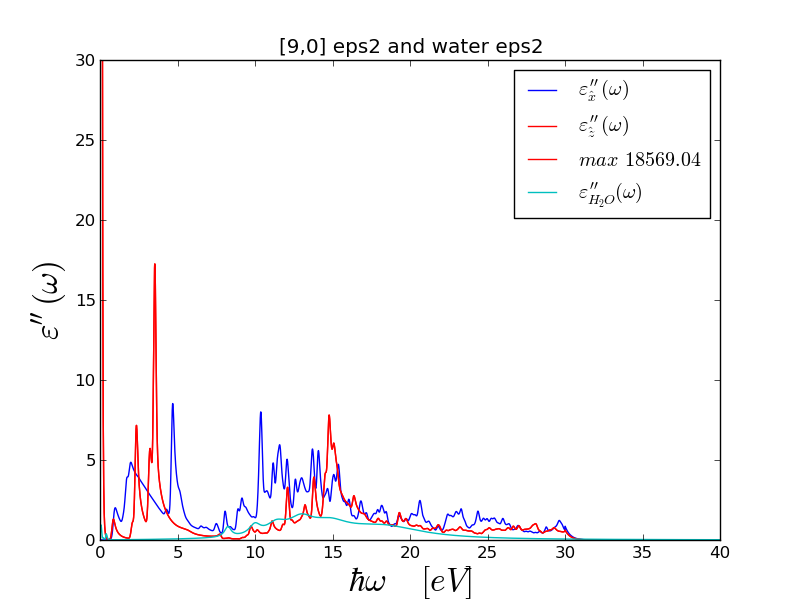
\includegraphics[width=1.4\textwidth]{prop_plots/90w90_eps2.png} (a)
\end{center}
\end{minipage}
\hskip 43pt
\begin{minipage}[b]{0.40\textwidth}
\begin{center}
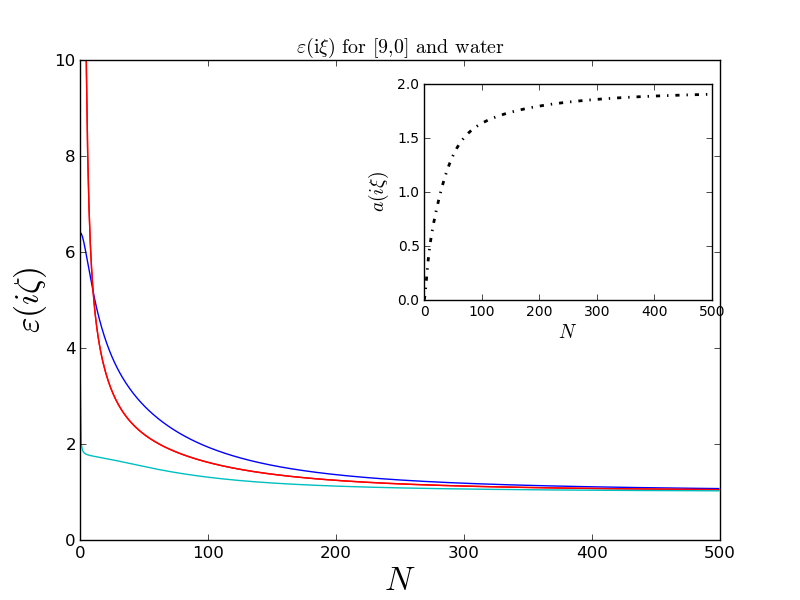
\includegraphics[width=1.4\textwidth]{prop_plots/90w90_eiz.png} (b)
\end{center}
\end{minipage}
\caption{(a) Imaginary dielectric response spectrum, (b) dispersion spectrum and anistropy measure (inset)}
\label{eiz91}
\end{center}
\end{figure*} 

%%%%%%%%%EPS2 and Aiz%%%%%%%%%%%%%%%%%%%%%%%%%%%%%%%%%%%%%%%%%%%%%%%%
\section{[9,1] dielectric response spectrum, dispersion spectrum, and anisotropy measure}
Relative anisotropy measures in the parallel and perpendicular direction are given by
\begin{equation}
\Delta_{\perp}=\frac{{\epsilon^{c}}_{\perp}-\epsilon_{m}}{{\epsilon^{c}}_{\perp}+\epsilon_{m}}\qquad\Delta_{\parallel}=\frac{{\epsilon^{c}}_{\parallel}-\epsilon_{m}}{\epsilon_{m}}.
\label{anisoind}
\end{equation}

Ratio of anisotropy measures

\begin{equation}
a_{1,2}(i \omega_n) = \frac{2 \Delta_{\perp}^{(1,2)}(i \omega_n)}{\Delta_{\parallel}^{(1,2)}(i \omega_n)} = 2 \frac{({{\epsilon^{c}}_{\perp}}^{(1,2)}(i \omega_n) -\epsilon_{m}(i \omega_n)) \epsilon_{m}(i \omega_n)}{({{\epsilon^{c}}_{\perp}}^{(1,2)}(i \omega_n)+\epsilon_{m}(i \omega_n)) ({{\epsilon^{c}}_{\parallel}}^{(1,2)}(i \omega_n) -\epsilon_{m}(i \omega_n))}
\label{eq:adef}
\end{equation}

\begin{figure*}[t!]
\begin{center}
\begin{minipage}[b]{0.40\textwidth}
\begin{center}
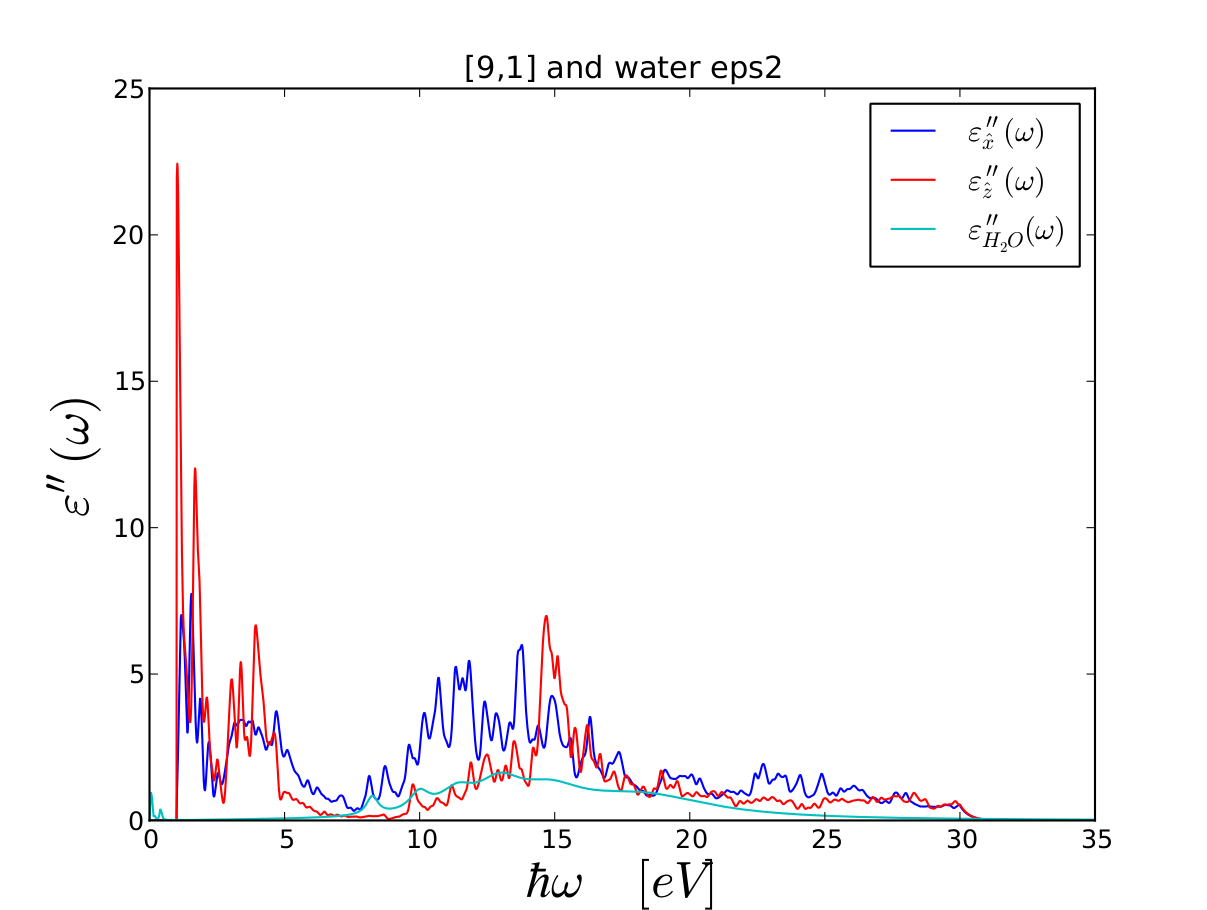
\includegraphics[width=1.4\textwidth]{prop_plots/91w91_eps2.png} (a)
\end{center}
\end{minipage}
\hskip 43pt
\begin{minipage}[b]{0.40\textwidth}
\begin{center}
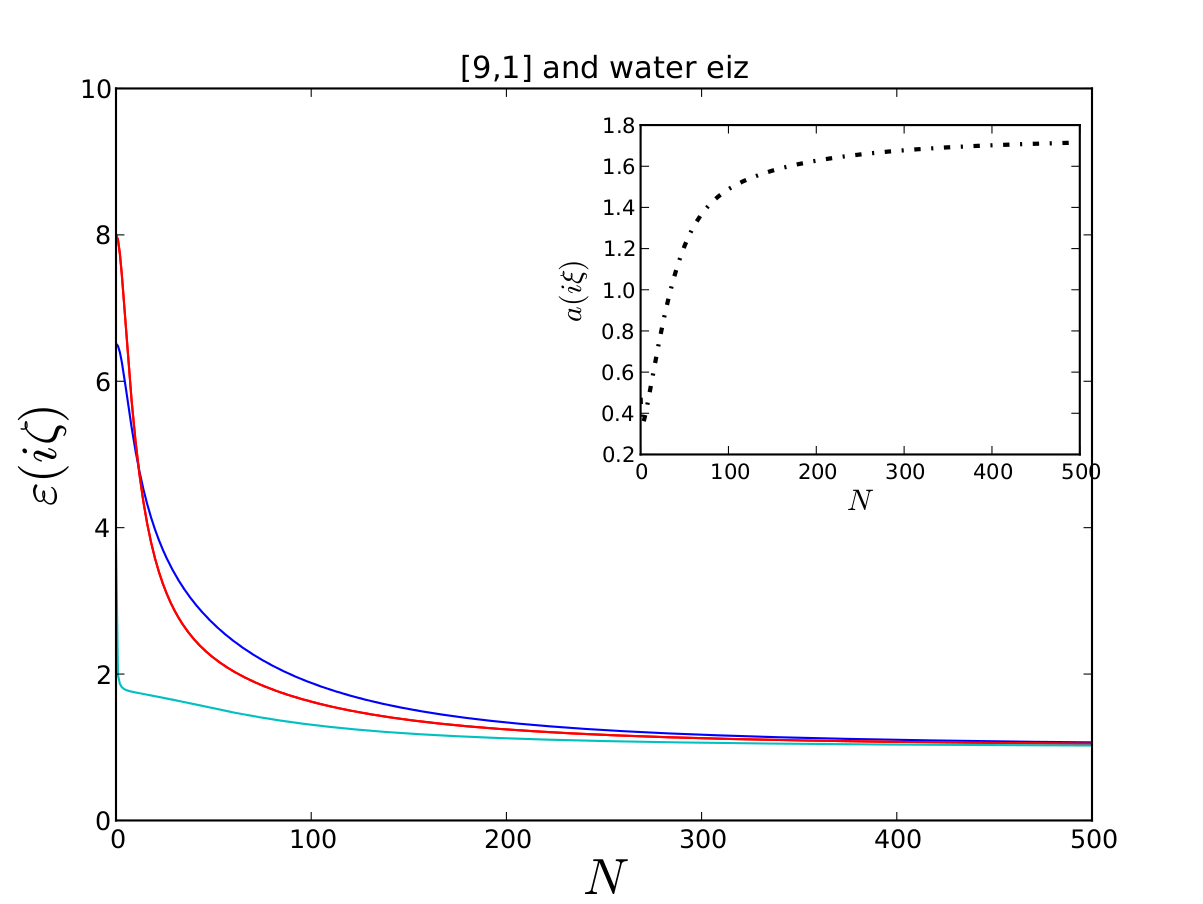
\includegraphics[width=1.4\textwidth]{prop_plots/91w91_eiz.png} (b)
\end{center}
\end{minipage}
\caption{(a) Imaginary dielectric response spectrum, (b) dispersion spectrum and anistropy measure (inset)}
\label{eiz91}
\end{center}
\end{figure*} 

%%%%%%%%%EPS2 and Aiz%%%%%%%%%%%%%%%%%%%%%%%%%%%%%%%%%%%%%%%%%%%%%%%%
\section{[9,3] dielectric response spectrum, dispersion spectrum, and anisotropy measure}
Relative anisotropy measures in the parallel and perpendicular direction are given by

\begin{equation}
\Delta_{\perp}=\frac{{\epsilon^{c}}_{\perp}-\epsilon_{m}}{{\epsilon^{c}}_{\perp}+\epsilon_{m}}\qquad\Delta_{\parallel}=\frac{{\epsilon^{c}}_{\parallel}-\epsilon_{m}}{\epsilon_{m}}.
\label{anisoind}
\end{equation}

Ratio of anisotropy measures
\begin{equation}
a_{1,2}(i \omega_n) = \frac{2 \Delta_{\perp}^{(1,2)}(i \omega_n)}{\Delta_{\parallel}^{(1,2)}(i \omega_n)} = 2 \frac{({{\epsilon^{c}}_{\perp}}^{(1,2)}(i \omega_n) -\epsilon_{m}(i \omega_n)) \epsilon_{m}(i \omega_n)}{({{\epsilon^{c}}_{\perp}}^{(1,2)}(i \omega_n)+\epsilon_{m}(i \omega_n)) ({{\epsilon^{c}}_{\parallel}}^{(1,2)}(i \omega_n) -\epsilon_{m}(i \omega_n))}
\label{eq:adef}
\end{equation}
\begin{figure*}[t!]
\begin{center}
\begin{minipage}[b]{0.40\textwidth}
\begin{center}
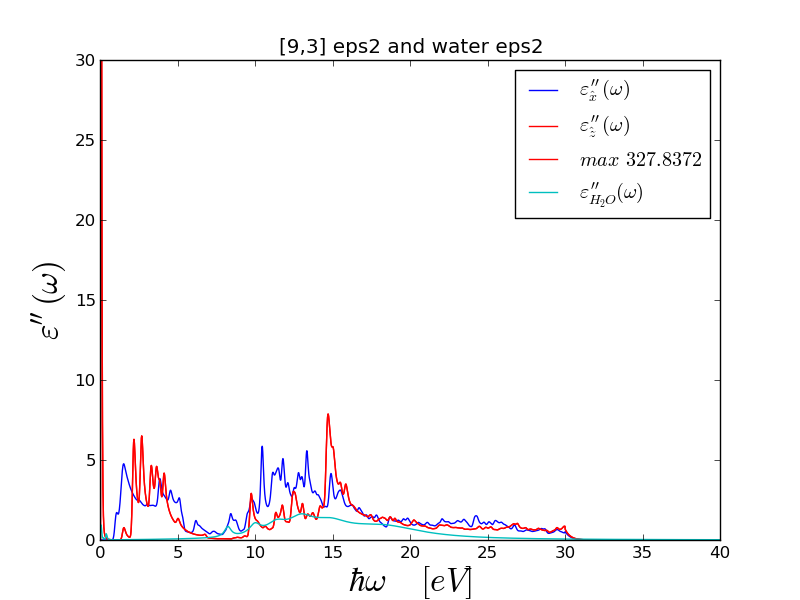
\includegraphics[width=1.4\textwidth]{prop_plots/93w93_eps2.png} (a)
\end{center}
\end{minipage}
\hskip 43pt
\begin{minipage}[b]{0.40\textwidth}
\begin{center}
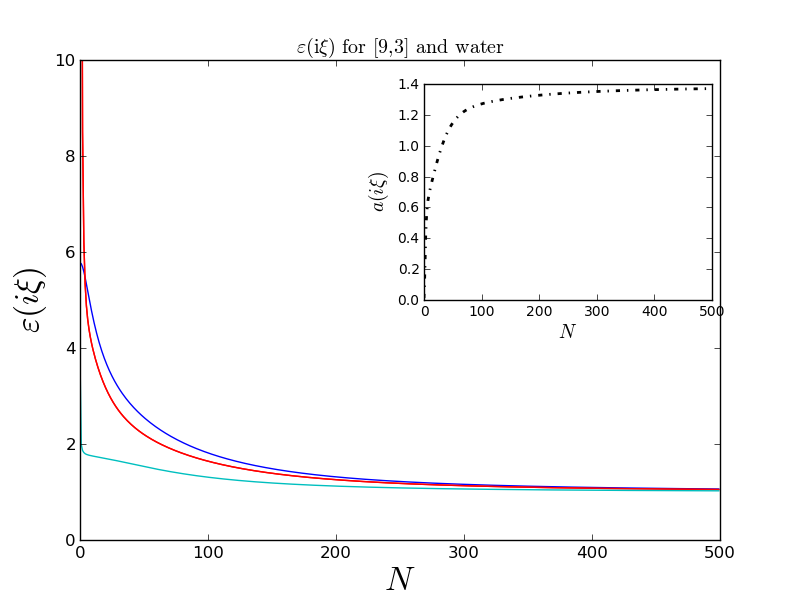
\includegraphics[width=1.4\textwidth]{prop_plots/93w93_eiz.png} (b)
\end{center}
\end{minipage}
\caption{(a) Imaginary dielectric response spectrum, (b) dispersion spectrum and anistropy measure (inset)}
\label{eiz91}
\end{center}
\end{figure*} 

%%%%%%%%%EPS2 and Aiz%%%%%%%%%%%%%%%%%%%%%%%%%%%%%%%%%%%%%%%%%%%%%%%%
\section{[29,0] dielectric response spectrum, dispersion spectrum, and anisotropy measure}
Relative anisotropy measures in the parallel and perpendicular direction are given by

\begin{equation}
\Delta_{\perp}=\frac{{\epsilon^{c}}_{\perp}-\epsilon_{m}}{{\epsilon^{c}}_{\perp}+\epsilon_{m}}\qquad\Delta_{\parallel}=\frac{{\epsilon^{c}}_{\parallel}-\epsilon_{m}}{\epsilon_{m}}.
\label{anisoind}
\end{equation}

Ratio of anisotropy measures

\begin{equation}
a_{1,2}(i \omega_n) = \frac{2 \Delta_{\perp}^{(1,2)}(i \omega_n)}{\Delta_{\parallel}^{(1,2)}(i \omega_n)} = 2 \frac{({{\epsilon^{c}}_{\perp}}^{(1,2)}(i \omega_n) -\epsilon_{m}(i \omega_n)) \epsilon_{m}(i \omega_n)}{({{\epsilon^{c}}_{\perp}}^{(1,2)}(i \omega_n)+\epsilon_{m}(i \omega_n)) ({{\epsilon^{c}}_{\parallel}}^{(1,2)}(i \omega_n) -\epsilon_{m}(i \omega_n))}
\label{eq:adef}
\end{equation}

\begin{figure*}[t!]
\begin{center}
\begin{minipage}[b]{0.40\textwidth}
\begin{center}
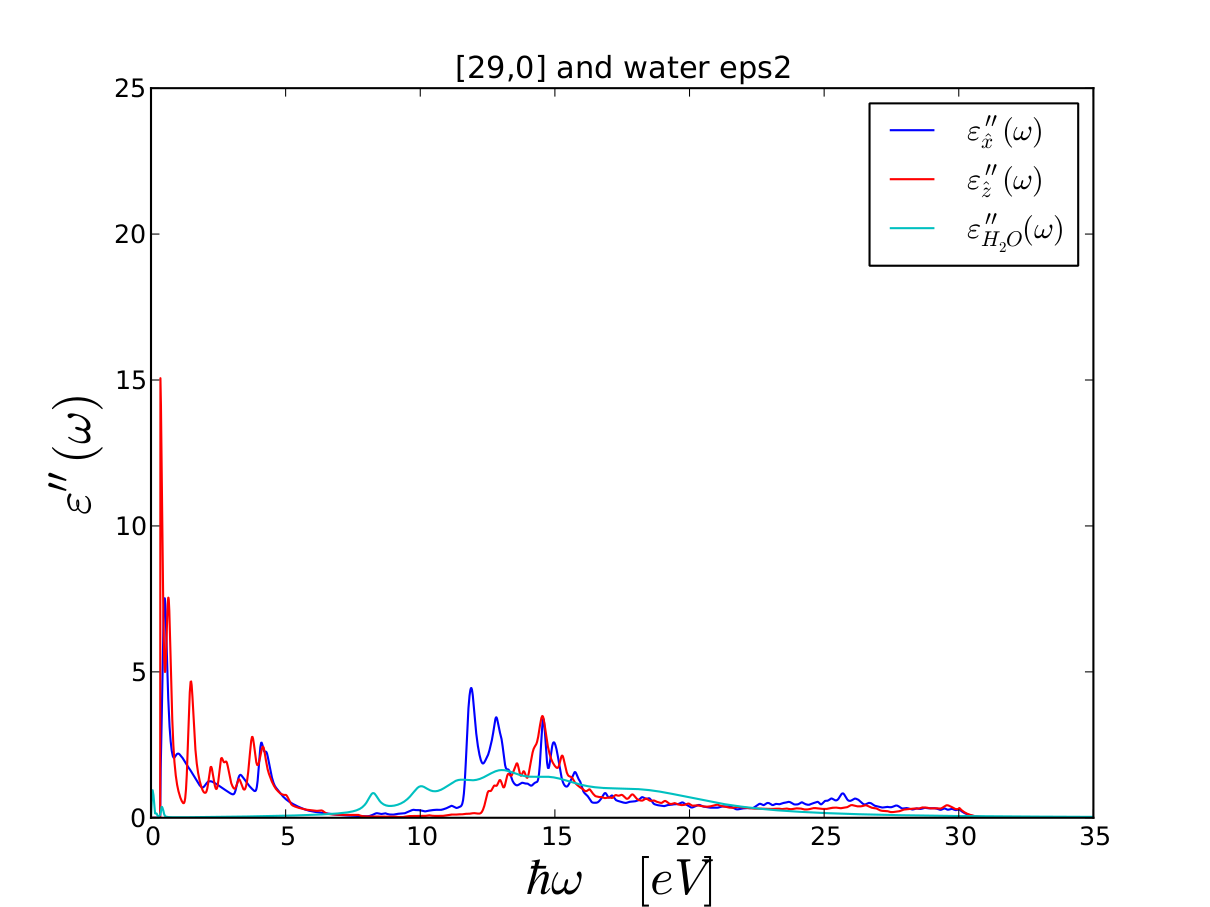
\includegraphics[width=1.4\textwidth]{prop_plots/290w290_eps2.png} (a)
\end{center}
\end{minipage}
\hskip 43pt
\begin{minipage}[b]{0.40\textwidth}
\begin{center}
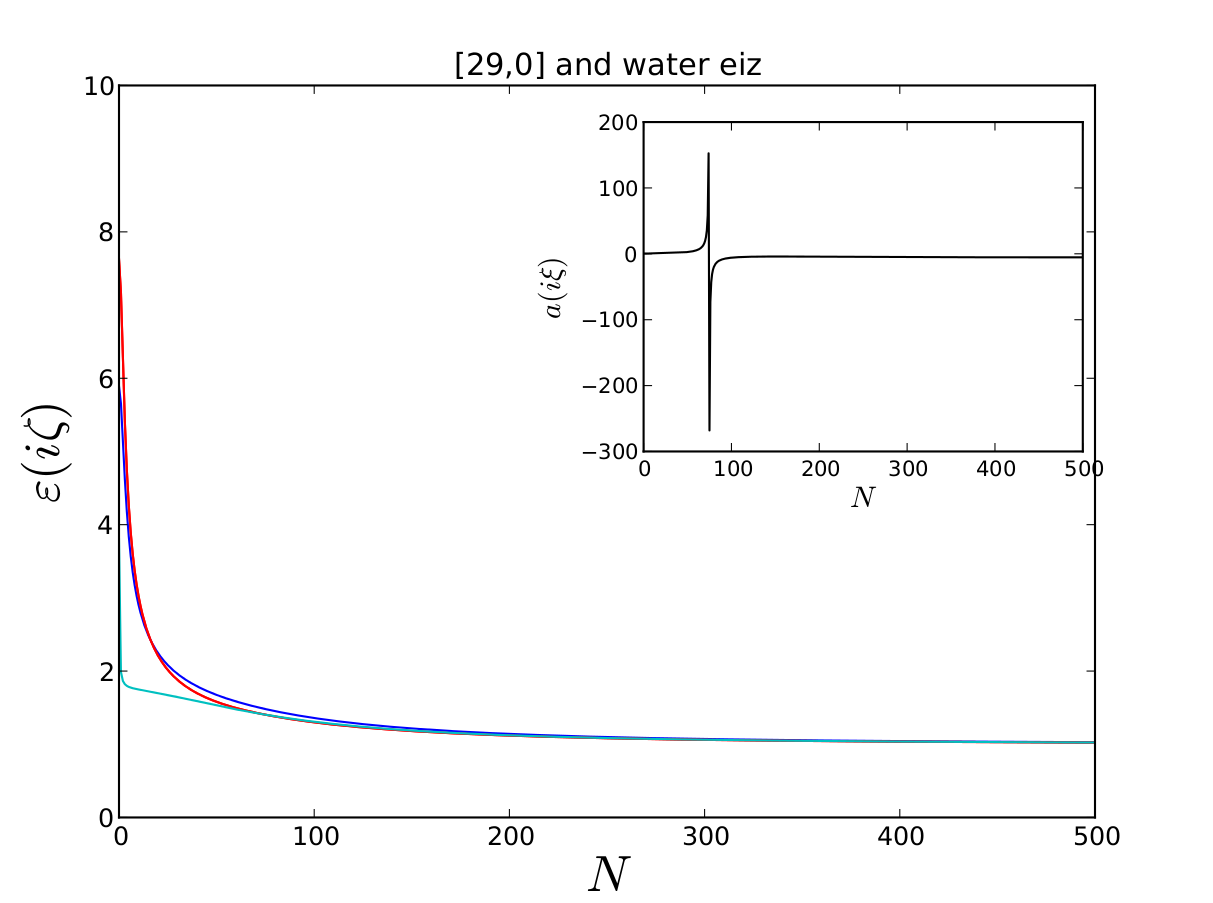
\includegraphics[width=1.4\textwidth]{prop_plots/290w290_eiz.png} (b)
\end{center}
\end{minipage}
\caption{(a) Imaginary dielectric response spectrum, (b) dispersion spectrum and anisotropy measure (inset)}
\label{eiz290}
\end{center}
\end{figure*} 

%%%%%%%%%%%%%%%%%%%%%%%%%%%%%%%%%% HAMAKERS %%%%%%%%%%%%%%%%%%%%%%%%%%%%%%%%%%%%
%\chapter{Fully retarded Hamaker Coefficients}
%
%\section{[6,5]}
%\subsection{[6,5] terms of Matsubara sum}
%\begin{figure*}[t!]
%\begin{center}
%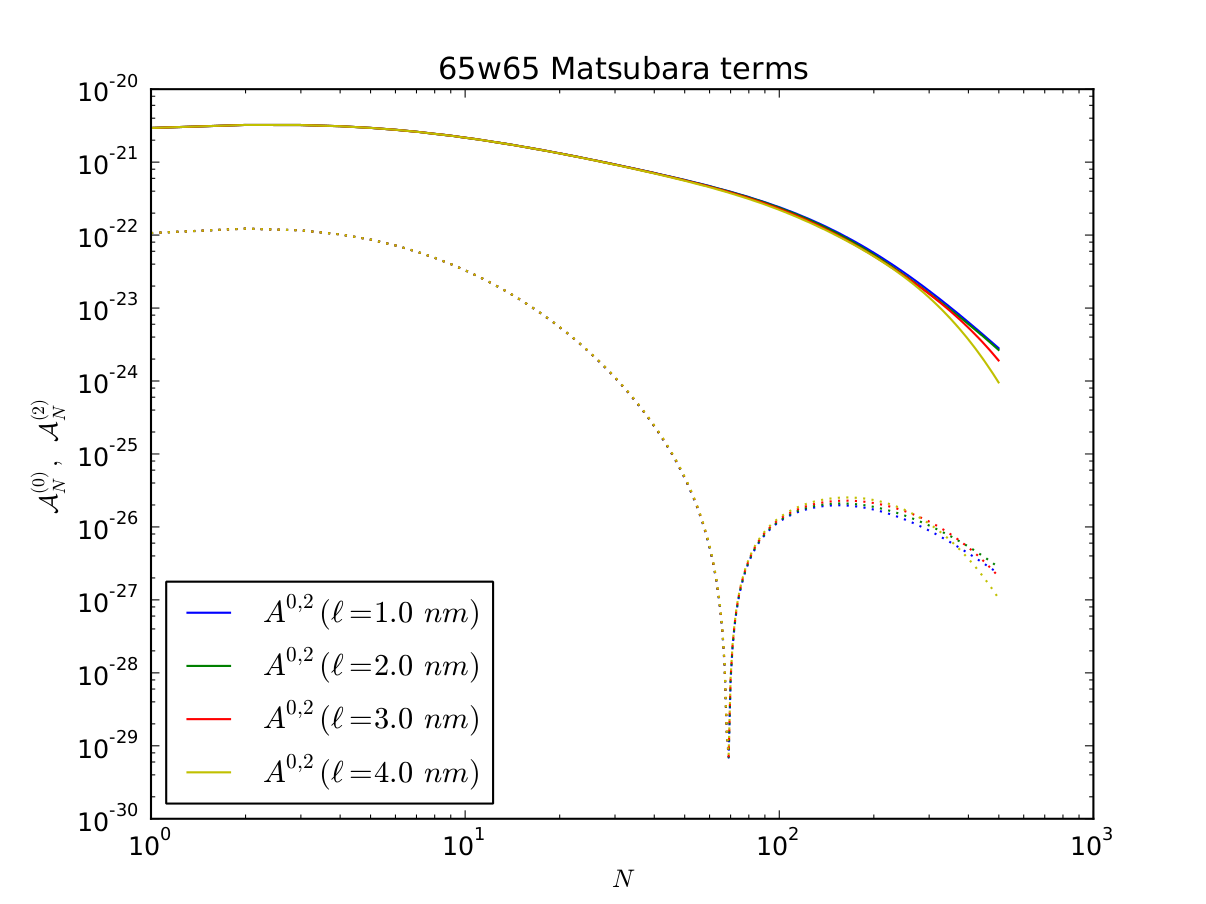
\includegraphics[width=1.2\textwidth]{plots/65_A_vs_n.png}
%\hskip 43pt
%\caption{Terms contributing to Matsubara sum as a function of N}
%\label{eiz65}
%\end{center}
%\end{figure*} 
%
%\subsection{[6,5] Log-log plot of $\mathcal{A}^{(0)}$ and $\mathcal{A}^{(2)}$ }
%\begin{figure*}[t!]
%\begin{center}
%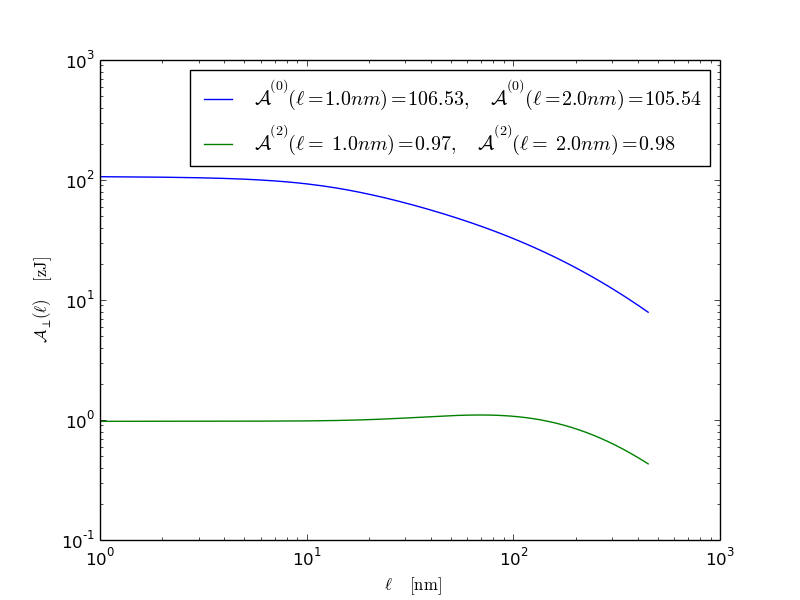
\includegraphics[width=1.2\textwidth]{plots/140322_65w65_HCs_perpendicular_ret.png}
%\hskip 43pt
%\caption{Full result} 
%\label{eiz65}
%\end{center}
%\end{figure*} 
%
%%\subsection{[6,5] Semi-log plot of $\mathcal{A}^{(0)}$ and $\mathcal{A}^{(2)}$ }
%%\begin{figure*}[t!]
%%\begin{center}
%%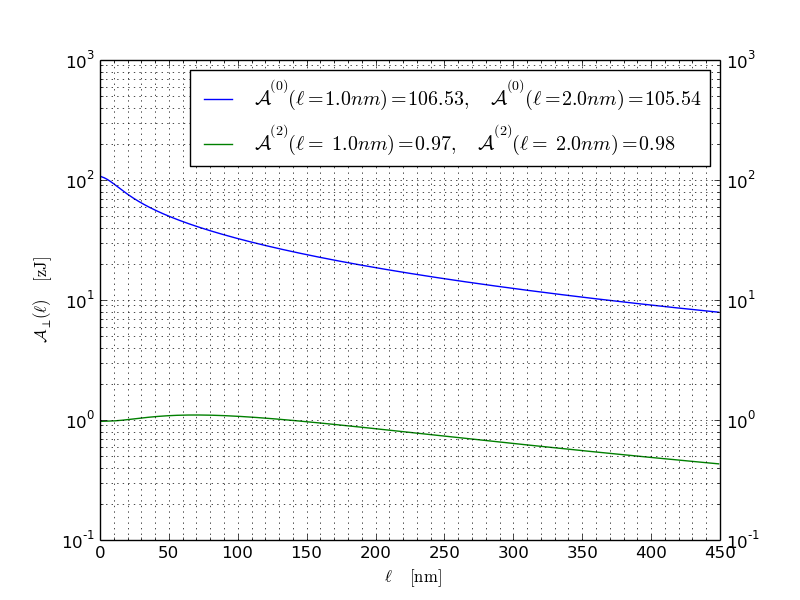
\includegraphics[width=1.2\textwidth]{plots/140322_65w65_HCs_semilog_perpendicular_ret.png}
%%\hskip 43pt
%%\caption{Full result using Eqs.\ref{pars-31},\ref{pars-31-g} (a) Anisotropic response functions for CG-10 DNA and water. The DNA response functions in the x and y directions were used as perpendicular and parallel inputs, respectively.  CG-10 and water eps2 data was provided by Dan Dryden. CG-10 data scales Wai-Yim's calculations by 4.94 and is assumed to include Na (more info in Dan Dryden email sent to us on Nov. 8, 2013).  Water data was built from lorentz oscillators R.H.French,J.Amer.Ceram Soc.,83,9,2117-46(2000), H.D.Ackler, et al,J.Coll.Interface Sci.179,46.
%%(b) Anisotropy metric $a_{1,2}(i\zeta_n)$ using Eq.\ref{eq:adef}, compares the anisotropy of the  cylinders (DNA) to their intervening material, water for the terms contruting to the Matsubara sum.}
%%\label{eiz65}
%%\end{center}
%%\end{figure*} 
%
%\section{[9,1]}
%\subsection{[9,1] terms of Matsubara sum}
%
%\begin{figure*}[t!]
%\begin{center}
%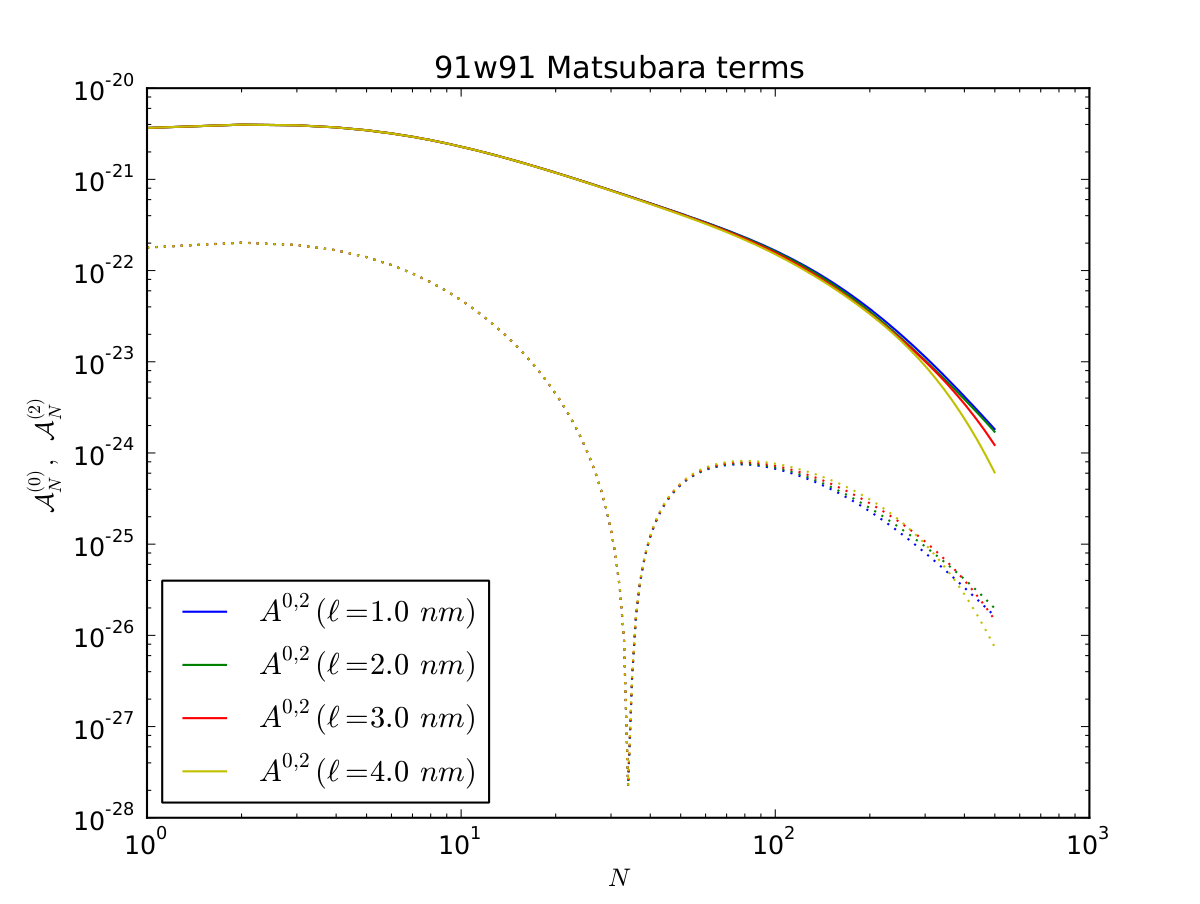
\includegraphics[width=1.2\textwidth]{plots/91_A_vs_n.png}
%\hskip 43pt
%\caption{Terms contributing to Matsubara sum as a function of N}
%\label{eiz65}
%\end{center}
%\end{figure*} 
%
%\subsection{[9,1] Log-log plot of $\mathcal{A}^{(0)}$ and $\mathcal{A}^{(2)}$ }
%\begin{figure*}[t!]
%\begin{center}
%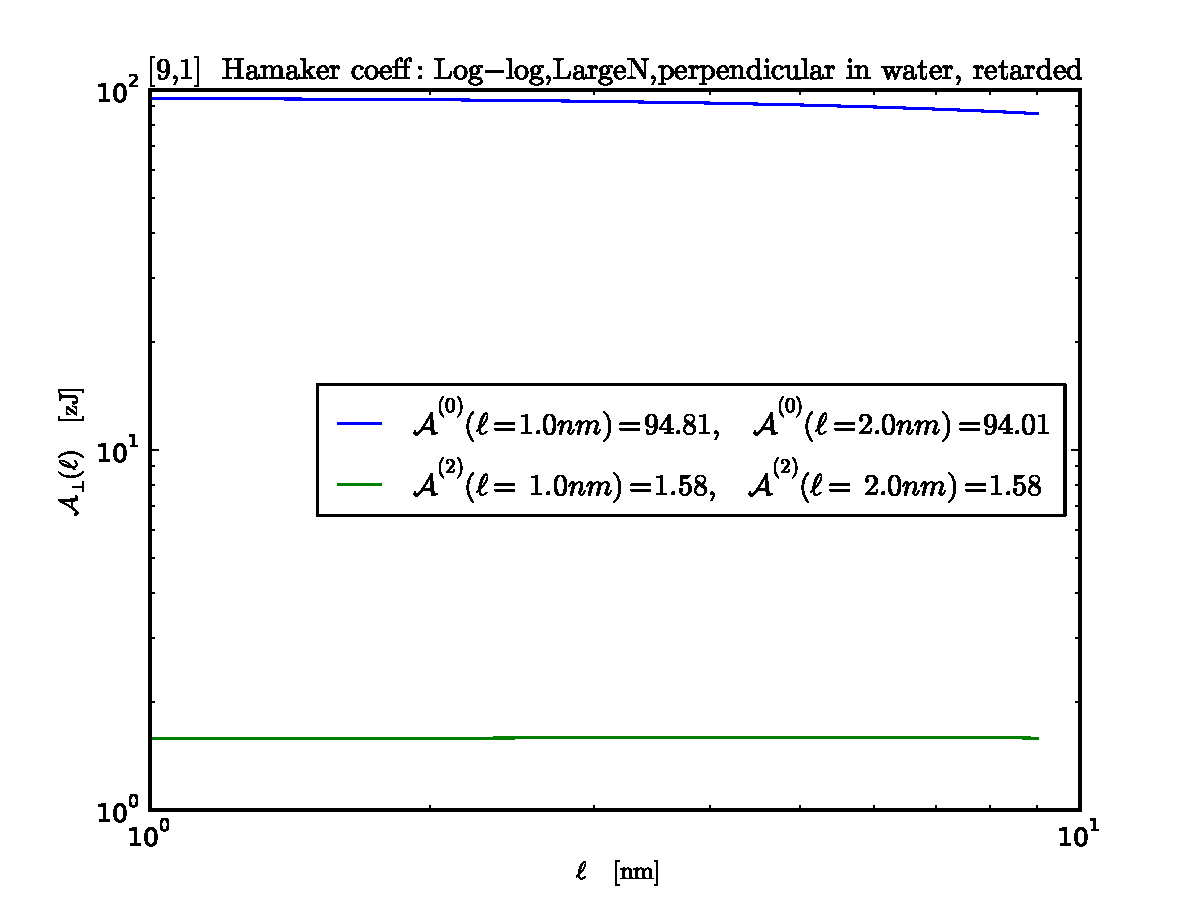
\includegraphics[width=1.2\textwidth]{plots/140322_91w91_HCs_perpendicular_ret.png}
%\hskip 43pt
%\caption{Full result}
%\label{eiz65}
%\end{center}
%\end{figure*} 
%
%\subsection{[9,1] Semi-log plot of $\mathcal{A}^{(0)}$ and $\mathcal{A}^{(2)}$ }
%\begin{figure*}[t!]
%\begin{center}
%\includegraphics[width=1.2\textwidth]{plots/140322_91w91_semilog_HCs_perpendicular_ret.png}
%\hskip 43pt
%\caption{Full result}
%\label{eiz65}
%\end{center}
%\end{figure*} 
%
%\section{[29,0]}
%\subsection{[29,0] terms of Matsubara sum}
%
%\begin{figure*}[t!]
%\begin{center}
%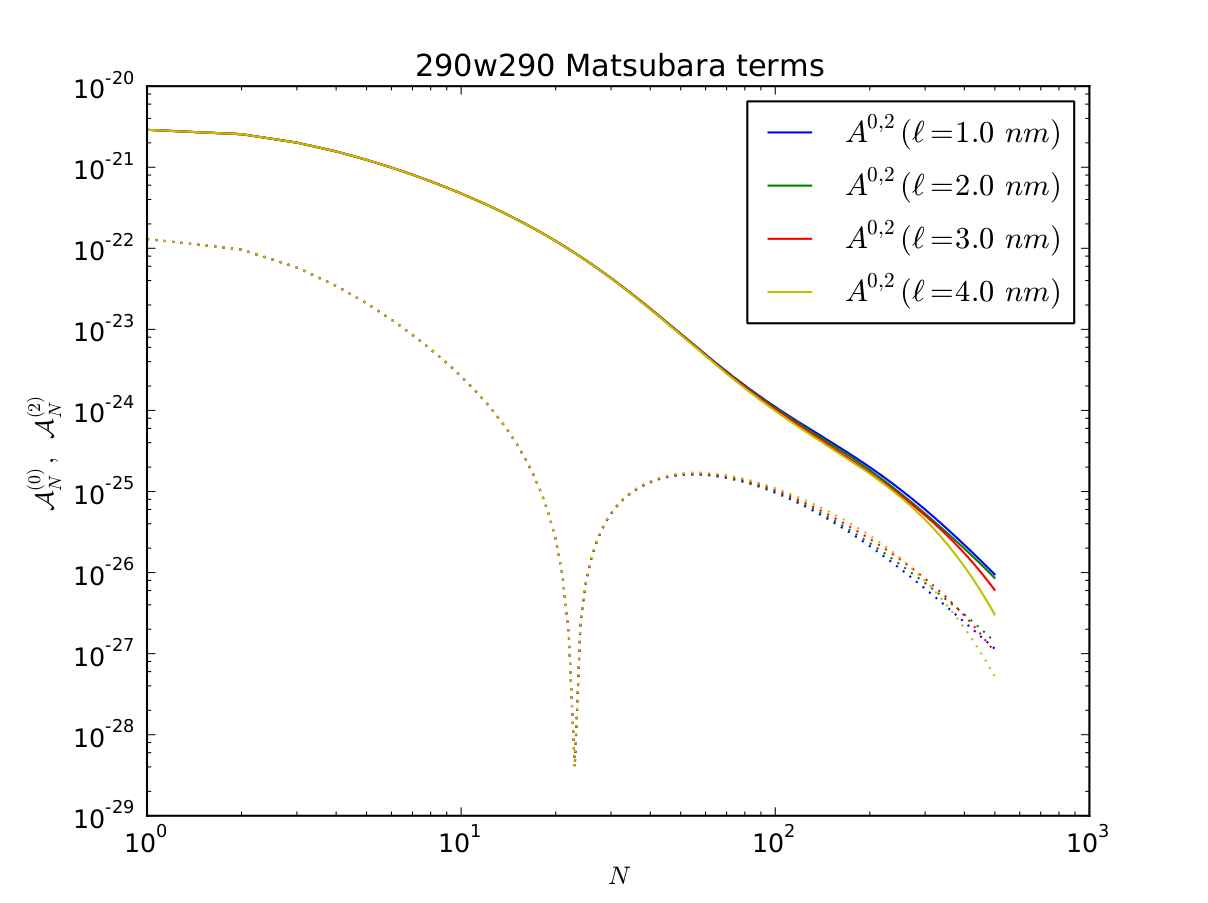
\includegraphics[width=1.2\textwidth]{plots/290_A_vs_n.png}
%\hskip 43pt
%\caption{Full result}
%\label{eiz65}
%\end{center}
%\end{figure*} 
%
%\subsection{[29,0] Log-log plot of $\mathcal{A}^{(0)}$ and $\mathcal{A}^{(2)}$ }
%\begin{figure*}[t!]
%\begin{center}
%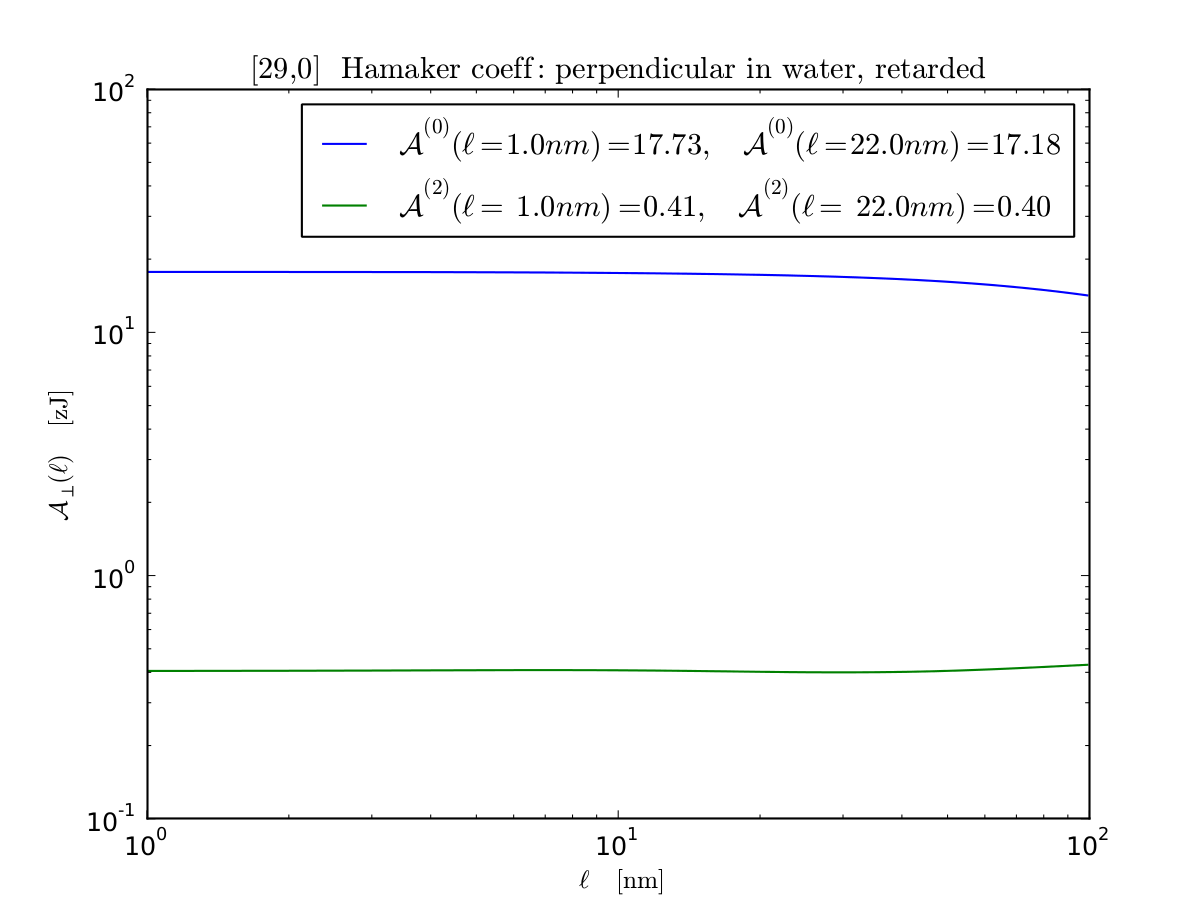
\includegraphics[width=1.2\textwidth]{plots/140322_290w290_HCs_perpendicular_ret.png}
%\hskip 43pt
%\caption{Full result}
%\label{eiz65}
%\end{center}
%\end{figure*} 
%
%\subsection{[29,0] Semi-log plot of $\mathcal{A}^{(0)}$ and $\mathcal{A}^{(2)}$ }
%\begin{figure*}[t!]
%\begin{center}
%\includegraphics[width=1.2\textwidth]{plots/140322_290w290_HCs_semilog_perpendicular_ret.png}
%\hskip 43pt
%\caption{Full result}
%\label{eiz65}
%\end{center}
%\end{figure*} 


%%%%%%%%%%%%%%%%%%%%%%%%%%%%%%%%%[6,5] HAMAKERS %%%%%%%%%%%%%%%%%%%%%%%%%%%%%%%
\chapter{Fully retarded Hamaker Coefficients for Matsubara Sum}
\section{Semi-conductor [6,5]}
\subsection{[6,5] terms of Matsubara sum}

We write the Hamaker coefficients as,
\begin{equation}
{\cal A}^{(0)}(\ell) = \frac{k_BT}{32}  {\sum_{n=0}^{\infty}}' \Delta_{1,\parallel} \Delta_{2,\parallel} ~p_n^{4}(\ell) ~\int_0^{\infty} t dt ~\frac{e^{- 2 p_n(\ell) \sqrt{t^{2} + 1}}}{(t^{2} + 1)} \tilde g^{(0)}(t, a_1(i \omega_n), a_2(i \omega_n))
\end{equation}
with
\begin{multline*}
\tilde g^{(0)}(t, a_1(i \omega_n), a_2(i \omega_n)) = \\ 
2 \left[ (1+3a_1)(1+3a_2) t^{4} + 2 (1+2a_1+2a_2+3a_1a_2) t^{2}  + 2(1+a_1)(1+a_2)\right]
\end{multline*}
and
\begin{equation}
{\cal A}^{(2)}(\ell) = \frac{k_BT}{32}  {\sum_{n=0}^{\infty}}' \Delta_{1,\parallel} \Delta_{2,\parallel} ~p_n^{4}(\ell) ~\int_0^{\infty} t dt ~\frac{e^{- 2 p_n(\ell) \sqrt{t^{2} + 1}}}{(t^{2} + 1)} \tilde g^{(2)}(t, a_1(i \omega_n), a_2(i \omega_n), \theta)
\end{equation}
with
\begin{equation*}
\tilde g^{(2)}(t, a_1(i \omega_n), a_2(i \omega_n), \theta) = (1-a_1)(1-a_2)(t^{2} + 2)^2
\label{befgqw}
\end{equation*}

Where
\begin{equation*}
p_n^{2}(\ell) =  \epsilon_m(i \omega_n) \frac{\omega_n^{2}}{c^{2}} \ell^{2},
\end{equation*}
\begin{equation*}
\Delta_{\perp}=\frac{{\epsilon^{c}}_{\perp}-\epsilon_{m}}{{\epsilon^{c}}_{\perp}+\epsilon_{m}}\qquad\Delta_{\parallel}=\frac{{\epsilon^{c}}_{\parallel}-\epsilon_{m}}{\epsilon_{m}},
\label{anisoind}
\end{equation*}
\begin{equation*}
a = \frac{2 \Delta_{\perp}}{\Delta_{\parallel}} = 2 \frac{({\epsilon^{c}}_{\perp}-\epsilon_{m}) \epsilon_{m}}{({\epsilon^{c}}_{\perp}+\epsilon_{m}) ({\epsilon^{c}}_{\parallel}-\epsilon_{m})}
\label{eq:adef}
\end{equation*}

For n = 0, we use
\begin{equation}
    {\cal A}_{n=0}^{(0)}(\ell) = \frac{1}{2} \frac{k_BT}{32}
    \Delta_{1,\parallel} \Delta_{2,\parallel} ~\int_0^{\infty} u^3 du\,\,
    e^{-2u}\,\,[2(1 + 3a_1)(1 + 3a_2) ]
\end{equation}
and
\begin{equation}
    {\cal A}_{n=0}^{(2)}(\ell) = \frac{1}{2} \frac{k_BT}{32}
    \Delta_{1,\parallel} \Delta_{2,\parallel} ~\int_0^{\infty} u^3 du\,\,
    e^{-2u}\,\,[(1 - a_1)(1 - a_2) ]
\end{equation}
where $u = Ql$.


\begin{figure*}[t!]
\begin{center}
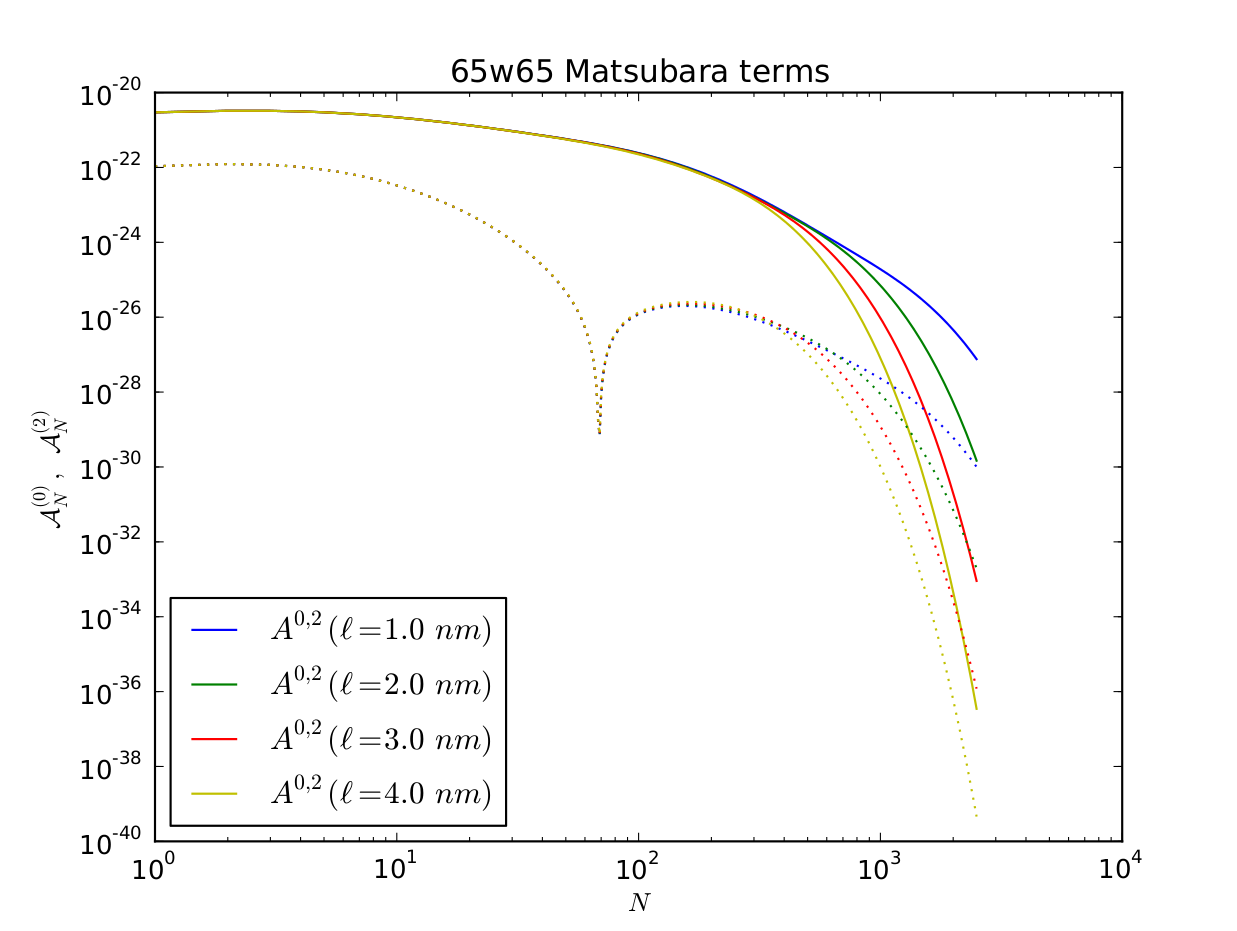
\includegraphics[width=1.2\textwidth]{large_N/65_A_vs_lrg_n.png}
\hskip 43pt
\caption{Terms contributing to Matsubara sum as a function of N}
\label{eiz65}
\end{center}
\end{figure*} 

%%%%%%%%%%%%%%%%%%%%%%%%%%%%%%%%% LOG A %%%%%%%%%%%%%%%%%%%
\subsection{[6,5] Log-log plot of $\mathcal{A}^{(0)}$ and $\mathcal{A}^{(2)}$ }
%\begin{}
\begin{equation}
{\cal A}^{(0)}(\ell) = \frac{k_BT}{32}  {\sum_{n=0}^{\infty}}' \Delta_{1,\parallel} \Delta_{2,\parallel} ~p_n^{4}(\ell) ~\int_0^{\infty} t dt ~\frac{e^{- 2 p_n(\ell) \sqrt{t^{2} + 1}}}{(t^{2} + 1)} \tilde g^{(0)}(t, a_1(i \omega_n), a_2(i \omega_n))
\end{equation}
%\end{}

with

\begin{multline*}
%\begin{equation}
%\begin{split}
\tilde g^{(0)}(t, a_1(i \omega_n), a_2(i \omega_n)) = \\ 
2 \left[ (1+3a_1)(1+3a_2) t^{4} + 2 (1+2a_1+2a_2+3a_1a_2) t^{2}  + 2(1+a_1)(1+a_2)\right]
%\end{split}
%\end{equation}
\end{multline*}

%\begin{equation}
%\tilde g^{(0)}(t, a_1(i \omega_n), a_2(i \omega_n)) = 2 \left[ (1+3a_1)(1+3a_2) t^{4} + 2 (1+2a_1+2a_2+3a_1a_2) t^{2}  + 2(1+a_1)(1+a_2)\right]
%\end{equation}

and

%\begin{}
\begin{equation}
{\cal A}^{(2)}(\ell) = \frac{k_BT}{32}  {\sum_{n=0}^{\infty}}' \Delta_{1,\parallel} \Delta_{2,\parallel} ~p_n^{4}(\ell) ~\int_0^{\infty} t dt ~\frac{e^{- 2 p_n(\ell) \sqrt{t^{2} + 1}}}{(t^{2} + 1)} \tilde g^{(2)}(t, a_1(i \omega_n), a_2(i \omega_n), \theta)
\end{equation}
%\end{}

with

\begin{equation}
\tilde g^{(2)}(t, a_1(i \omega_n), a_2(i \omega_n), \theta) = (1-a_1)(1-a_2)(t^{2} + 2)^2
\label{befgqw}
\end{equation}

\begin{figure*}[t!]
\begin{center}
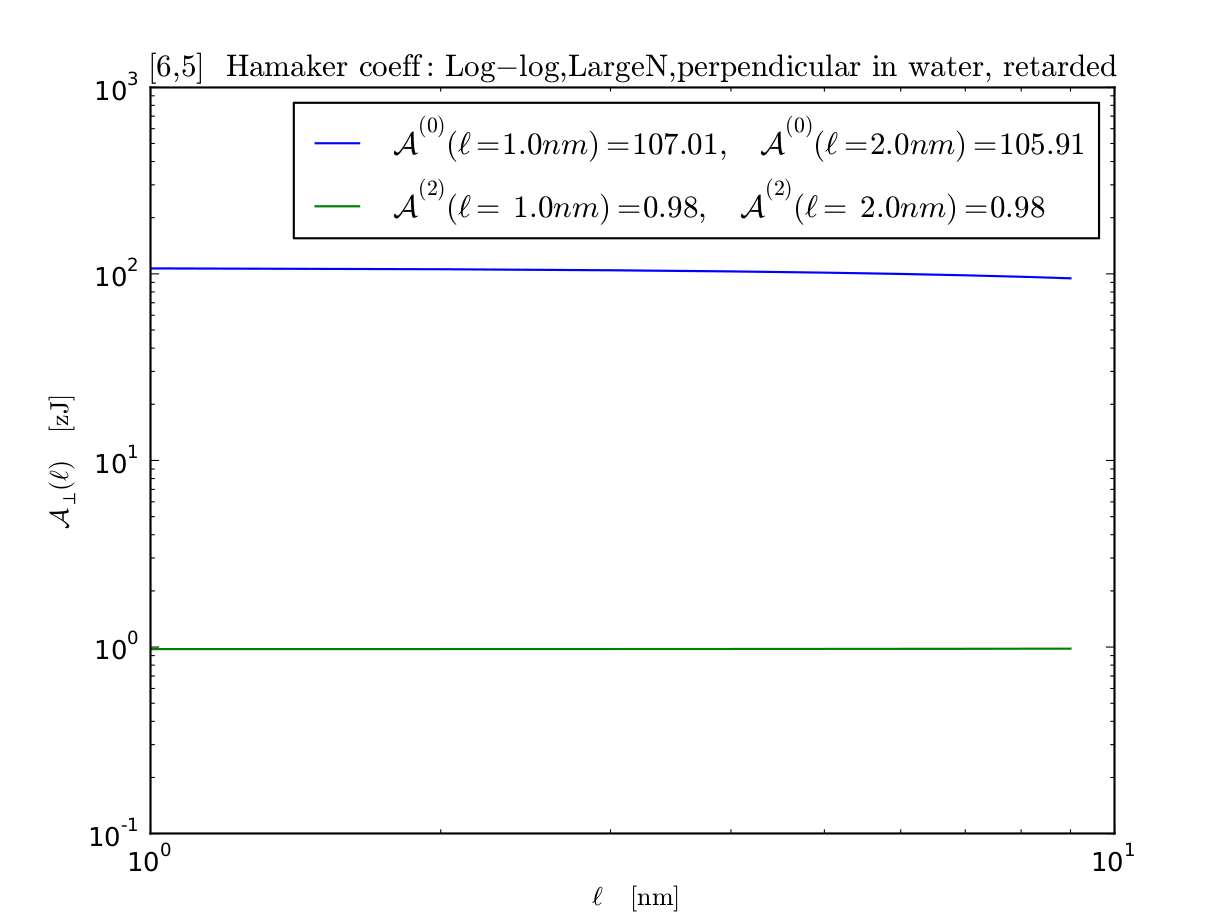
\includegraphics[width=1.2\textwidth]{large_N/140322_65w65_HCs_perpendicular_ret_lrg_n.png}
\hskip 43pt
\caption{Full result} 
\label{eiz65}
\end{center}
\end{figure*} 

%%%%%%%%%%%%%%%%%%%%%%%%%%%%%%%%% SEMILOG A %%%%%%%%%%%%%%%%
\subsection{[6,5] Semi-log plot of $\mathcal{A}^{(0)}$ and $\mathcal{A}^{(2)}$ }
%\begin{}
\begin{equation}
{\cal A}^{(0)}(\ell) = \frac{k_BT}{32}  {\sum_{n=0}^{\infty}}' \Delta_{1,\parallel} \Delta_{2,\parallel} ~p_n^{4}(\ell) ~\int_0^{\infty} t dt ~\frac{e^{- 2 p_n(\ell) \sqrt{t^{2} + 1}}}{(t^{2} + 1)} \tilde g^{(0)}(t, a_1(i \omega_n), a_2(i \omega_n))
\end{equation}
%\end{}

with

\begin{multline*}
%\begin{equation}
%\begin{split}
\tilde g^{(0)}(t, a_1(i \omega_n), a_2(i \omega_n)) = \\ 
2 \left[ (1+3a_1)(1+3a_2) t^{4} + 2 (1+2a_1+2a_2+3a_1a_2) t^{2}  + 2(1+a_1)(1+a_2)\right]
%\end{split}
%\end{equation}
\end{multline*}

%\begin{equation}
%\tilde g^{(0)}(t, a_1(i \omega_n), a_2(i \omega_n)) = 2 \left[ (1+3a_1)(1+3a_2) t^{4} + 2 (1+2a_1+2a_2+3a_1a_2) t^{2}  + 2(1+a_1)(1+a_2)\right]
%\end{equation}

and

\begin{equation}
{\cal A}^{(2)}(\ell) = \frac{k_BT}{32}  {\sum_{n=0}^{\infty}}' \Delta_{1,\parallel} \Delta_{2,\parallel} ~p_n^{4}(\ell) ~\int_0^{\infty} t dt ~\frac{e^{- 2 p_n(\ell) \sqrt{t^{2} + 1}}}{(t^{2} + 1)} \tilde g^{(2)}(t, a_1(i \omega_n), a_2(i \omega_n), \theta)
\end{equation}

with

\begin{equation}
\tilde g^{(2)}(t, a_1(i \omega_n), a_2(i \omega_n), \theta) = (1-a_1)(1-a_2)(t^{2} + 2)^2
\label{befgqw}
\end{equation}

\begin{figure*}[t!]
\begin{center}
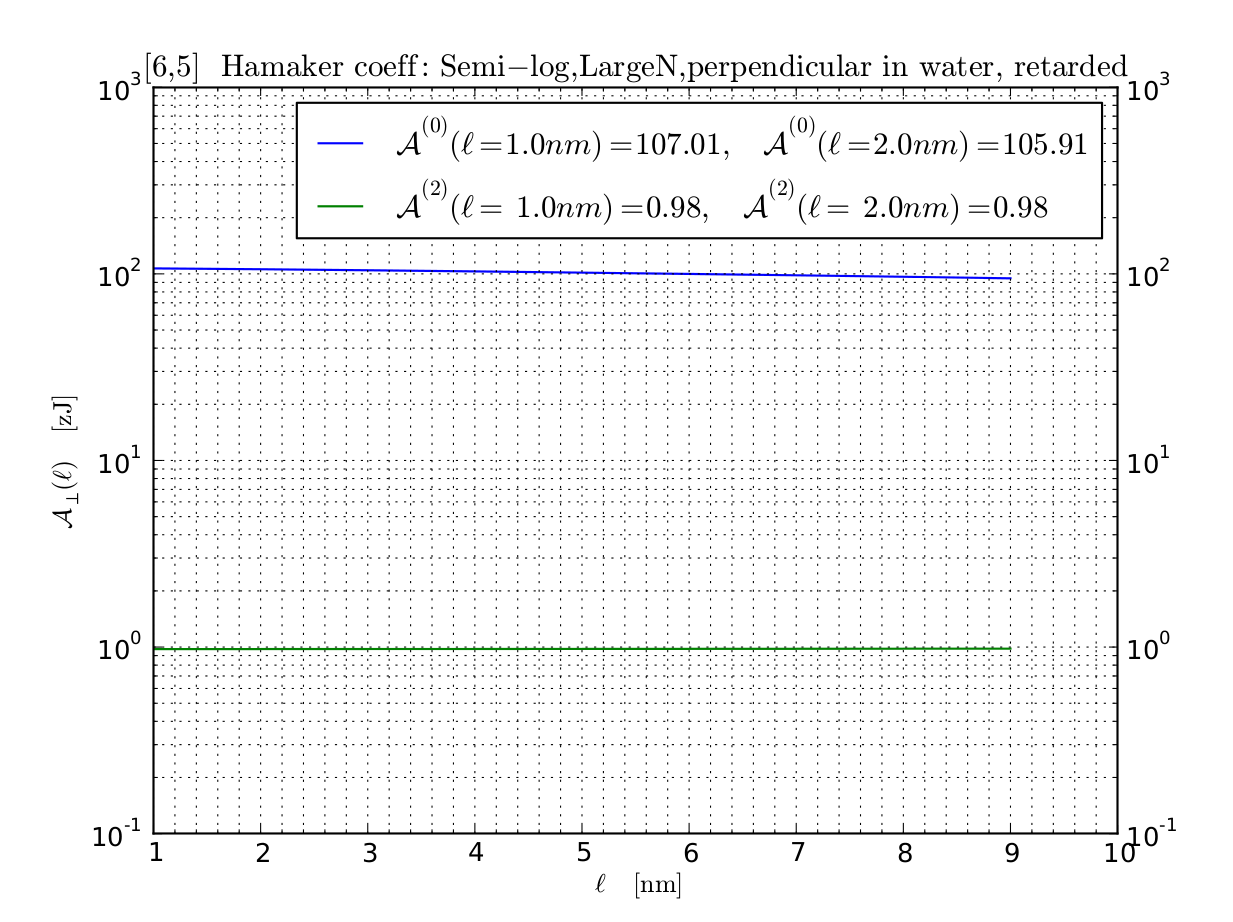
\includegraphics[width=1.2\textwidth]{large_N/140322_65w65_HCs_semilog_perpendicular_ret_lrg_n.png}
\hskip 43pt
\caption{Full result}
\label{eiz65}
\end{center}
\end{figure*} 

%%%%%%%%%%%%%%%%%%%%%%%%%%%%%%%%%[9,1] HAMAKERS %%%%%%%%%%%%%%%%%%%%%%%%%%%%%%%%
\section{Semi-conductor [9,1]}
\subsection{[9,1] terms of Matsubara sum}
\begin{equation}
{\cal A}^{(0)}(\ell) = \frac{k_BT}{32}  {\sum_{n=0}^{\infty}}' \Delta_{1,\parallel} \Delta_{2,\parallel} ~p_n^{4}(\ell) ~\int_0^{\infty} t dt ~\frac{e^{- 2 p_n(\ell) \sqrt{t^{2} + 1}}}{(t^{2} + 1)} \tilde g^{(0)}(t, a_1(i \omega_n), a_2(i \omega_n))
\end{equation}

with

\begin{multline*}
%\begin{equation}
%\begin{split}
\tilde g^{(0)}(t, a_1(i \omega_n), a_2(i \omega_n)) = \\ 
2 \left[ (1+3a_1)(1+3a_2) t^{4} + 2 (1+2a_1+2a_2+3a_1a_2) t^{2}  + 2(1+a_1)(1+a_2)\right]
%\end{split}
%\end{equation}
\end{multline*}

%\begin{equation}
%\tilde g^{(0)}(t, a_1(i \omega_n), a_2(i \omega_n)) = 2 \left[ (1+3a_1)(1+3a_2) t^{4} + 2 (1+2a_1+2a_2+3a_1a_2) t^{2}  + 2(1+a_1)(1+a_2)\right]
%\end{equation}

and

\begin{equation}
{\cal A}^{(2)}(\ell) = \frac{k_BT}{32}  {\sum_{n=0}^{\infty}}' \Delta_{1,\parallel} \Delta_{2,\parallel} ~p_n^{4}(\ell) ~\int_0^{\infty} t dt ~\frac{e^{- 2 p_n(\ell) \sqrt{t^{2} + 1}}}{(t^{2} + 1)} \tilde g^{(2)}(t, a_1(i \omega_n), a_2(i \omega_n), \theta)
\end{equation}

with

\begin{equation}
\tilde g^{(2)}(t, a_1(i \omega_n), a_2(i \omega_n), \theta) = (1-a_1)(1-a_2)(t^{2} + 2)^2
\label{befgqw}
\end{equation}


\begin{figure*}[t!]
\begin{center}
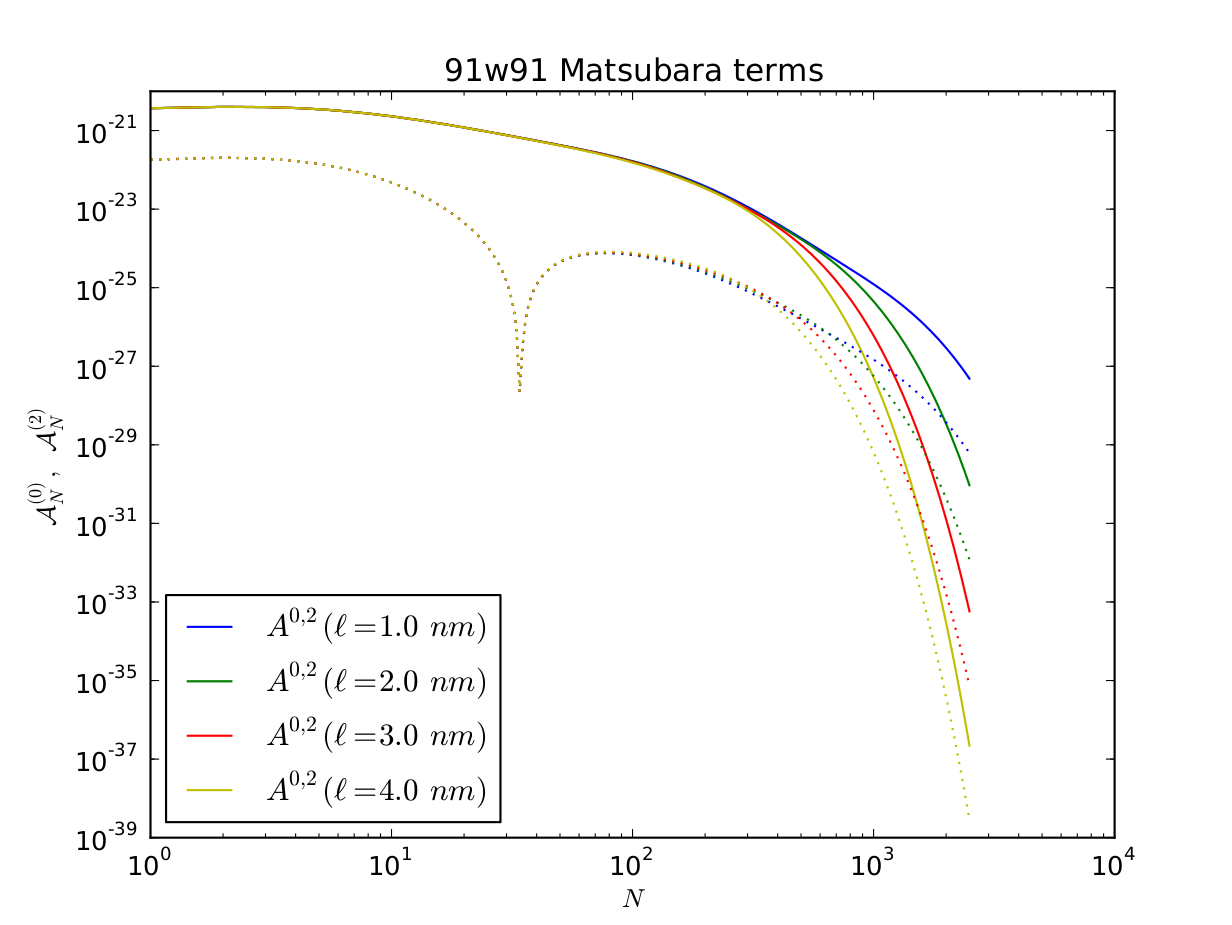
\includegraphics[width=1.2\textwidth]{large_N/91_A_vs_lrg_n.png}
\hskip 43pt
\caption{Terms contributing to Matsubara sum as a function of N}
\label{eiz65}
\end{center}
\end{figure*} 

%%%%%%%%%%%%%%%%%%%%%%%%%%%%%%%%% LOG A %%%%%%%%%%%%%%%%%%%%
\subsection{[9,1] Log-log plot of $\mathcal{A}^{(0)}$ and $\mathcal{A}^{(2)}$ }
\begin{equation}
{\cal A}^{(0)}(\ell) = \frac{k_BT}{32}  {\sum_{n=0}^{\infty}}' \Delta_{1,\parallel} \Delta_{2,\parallel} ~p_n^{4}(\ell) ~\int_0^{\infty} t dt ~\frac{e^{- 2 p_n(\ell) \sqrt{t^{2} + 1}}}{(t^{2} + 1)} \tilde g^{(0)}(t, a_1(i \omega_n), a_2(i \omega_n))
\end{equation}

with

\begin{multline*}
%\begin{equation}
%\begin{split}
\tilde g^{(0)}(t, a_1(i \omega_n), a_2(i \omega_n)) = \\ 
2 \left[ (1+3a_1)(1+3a_2) t^{4} + 2 (1+2a_1+2a_2+3a_1a_2) t^{2}  + 2(1+a_1)(1+a_2)\right]
%\end{split}
%\end{equation}
\end{multline*}

%\begin{equation}
%\tilde g^{(0)}(t, a_1(i \omega_n), a_2(i \omega_n)) = 2 \left[ (1+3a_1)(1+3a_2) t^{4} + 2 (1+2a_1+2a_2+3a_1a_2) t^{2}  + 2(1+a_1)(1+a_2)\right]
%\end{equation}

and

\begin{equation}
{\cal A}^{(2)}(\ell) = \frac{k_BT}{32}  {\sum_{n=0}^{\infty}}' \Delta_{1,\parallel} \Delta_{2,\parallel} ~p_n^{4}(\ell) ~\int_0^{\infty} t dt ~\frac{e^{- 2 p_n(\ell) \sqrt{t^{2} + 1}}}{(t^{2} + 1)} \tilde g^{(2)}(t, a_1(i \omega_n), a_2(i \omega_n), \theta)
\end{equation}

with

\begin{equation}
\tilde g^{(2)}(t, a_1(i \omega_n), a_2(i \omega_n), \theta) = (1-a_1)(1-a_2)(t^{2} + 2)^2
\label{befgqw}
\end{equation}

\begin{figure*}[t!]
\begin{center}
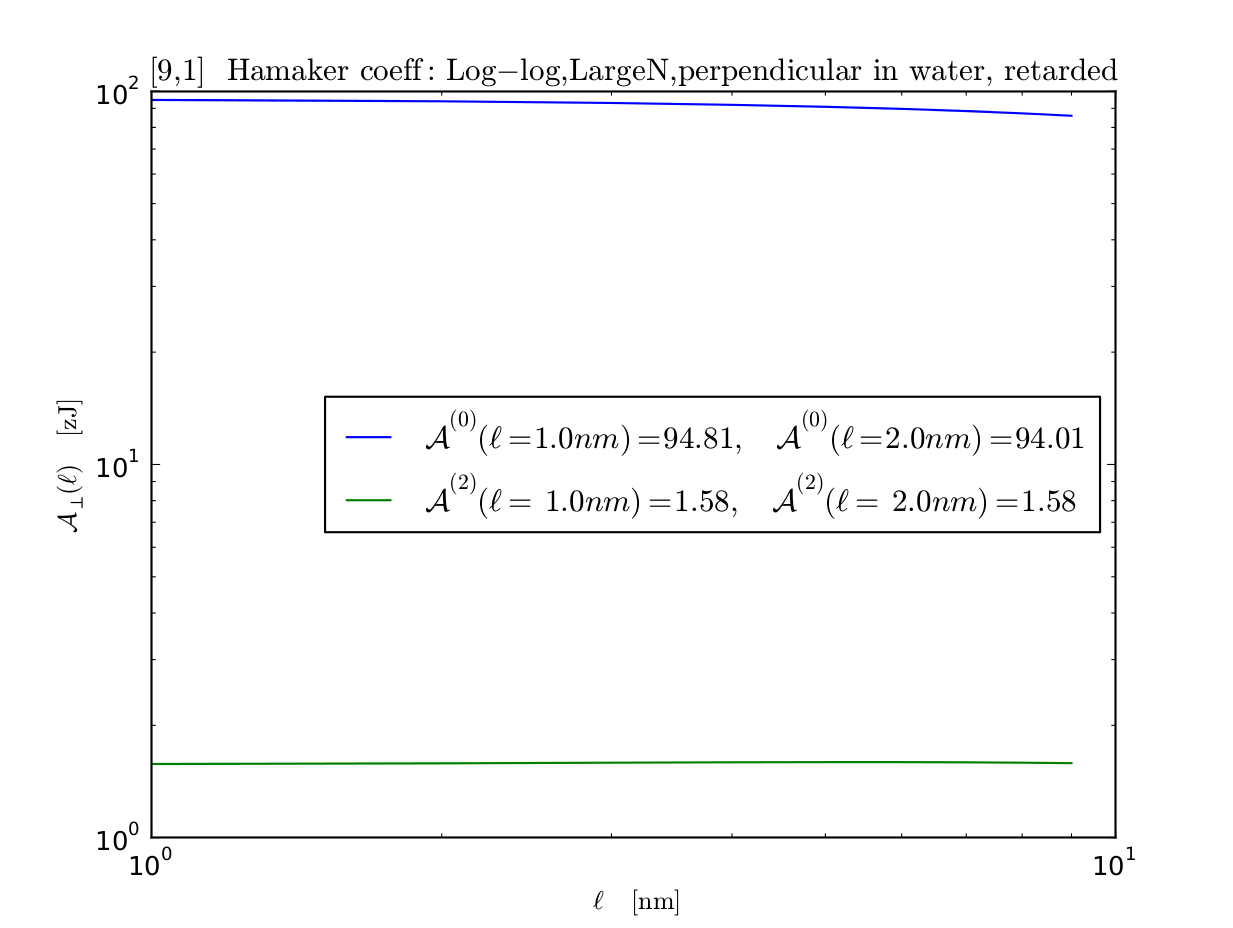
\includegraphics[width=1.2\textwidth]{large_N/140322_91w91_HCs_perpendicular_ret_lrg_n.png}
\hskip 43pt
\caption{Full result}
\label{eiz65}
\end{center}
\end{figure*} 

%%%%%%%%%%%%%%%%%%%%%%%%%%%%%%%%% SEMILOG A %%%%%%%%%%%%%%%%
\subsection{[9,1] Semi-log plot of $\mathcal{A}^{(0)}$ and $\mathcal{A}^{(2)}$ }
\begin{equation}
{\cal A}^{(0)}(\ell) = \frac{k_BT}{32}  {\sum_{n=0}^{\infty}}' \Delta_{1,\parallel} \Delta_{2,\parallel} ~p_n^{4}(\ell) ~\int_0^{\infty} t dt ~\frac{e^{- 2 p_n(\ell) \sqrt{t^{2} + 1}}}{(t^{2} + 1)} \tilde g^{(0)}(t, a_1(i \omega_n), a_2(i \omega_n))
\end{equation}

with

\begin{multline*}
%\begin{equation}
%\begin{split}
\tilde g^{(0)}(t, a_1(i \omega_n), a_2(i \omega_n)) = \\ 
2 \left[ (1+3a_1)(1+3a_2) t^{4} + 2 (1+2a_1+2a_2+3a_1a_2) t^{2}  + 2(1+a_1)(1+a_2)\right]
%\end{split}
%\end{equation}
\end{multline*}

%\begin{equation}
%\tilde g^{(0)}(t, a_1(i \omega_n), a_2(i \omega_n)) = 2 \left[ (1+3a_1)(1+3a_2) t^{4} + 2 (1+2a_1+2a_2+3a_1a_2) t^{2}  + 2(1+a_1)(1+a_2)\right]
%\end{equation}

and

\begin{equation}
{\cal A}^{(2)}(\ell) = \frac{k_BT}{32}  {\sum_{n=0}^{\infty}}' \Delta_{1,\parallel} \Delta_{2,\parallel} ~p_n^{4}(\ell) ~\int_0^{\infty} t dt ~\frac{e^{- 2 p_n(\ell) \sqrt{t^{2} + 1}}}{(t^{2} + 1)} \tilde g^{(2)}(t, a_1(i \omega_n), a_2(i \omega_n), \theta)
\end{equation}

with

\begin{equation}
\tilde g^{(2)}(t, a_1(i \omega_n), a_2(i \omega_n), \theta) = (1-a_1)(1-a_2)(t^{2} + 2)^2
\label{befgqw}
\end{equation}

\begin{figure*}[t!]
\begin{center}
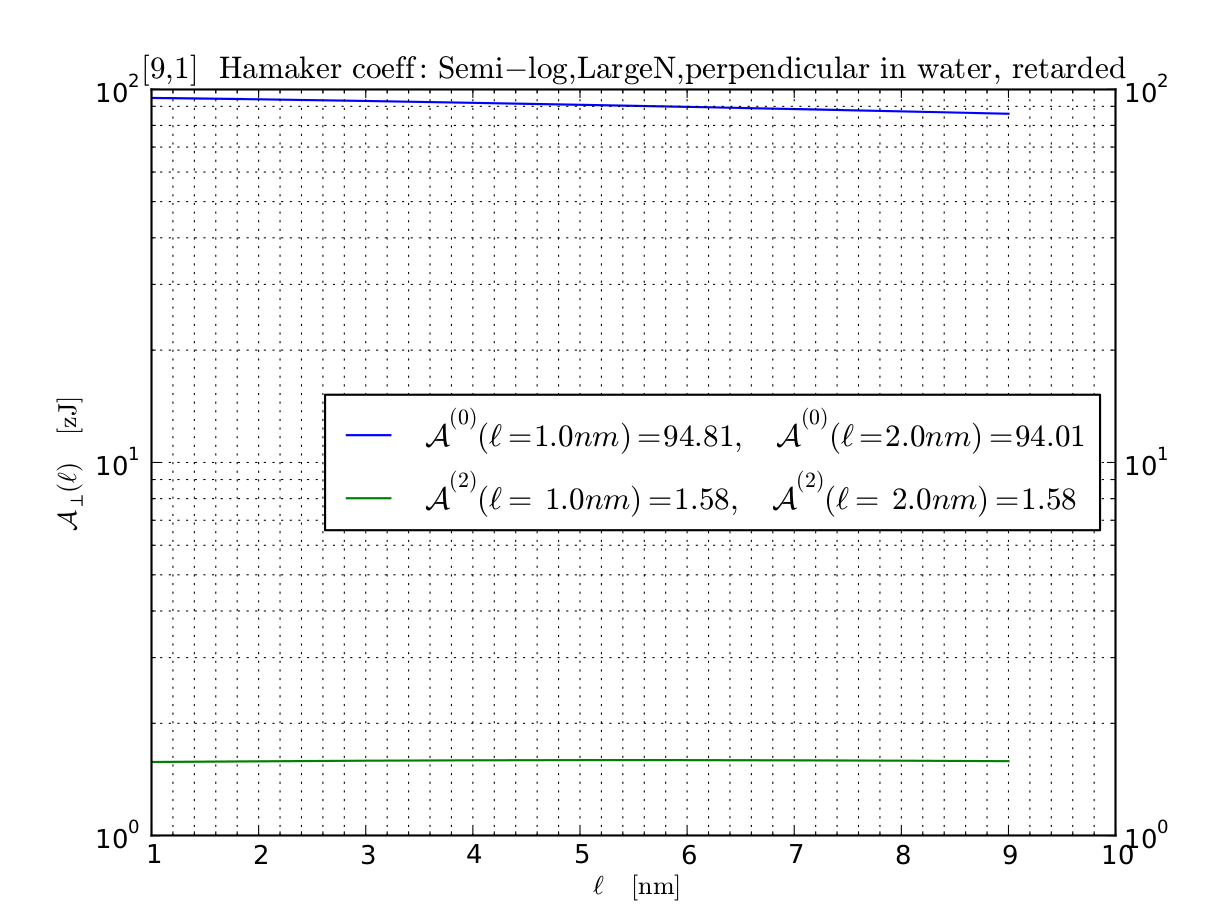
\includegraphics[width=1.2\textwidth]{large_N/140322_91w91_semilog_HCs_perpendicular_ret_lrg_n.png}
\hskip 43pt
\caption{Full result}
\label{eiz65}
\end{center}
\end{figure*} 

%%%%%%%%%%%%%%%%%%%%%%%%%%%%%%%%%[9,3] HAMAKERS %%%%%%%%%%%%%%%%%%%%%%%%%%%%%%%%
\section{First results for semi-metal [9,3]}
\subsection{[9,3] terms of unmodified Matsubara sum }
\begin{equation}
{\cal A}^{(0)}(\ell) = \frac{k_BT}{32}  {\sum_{n=0}^{\infty}}' \Delta_{1,\parallel} \Delta_{2,\parallel} ~p_n^{4}(\ell) ~\int_0^{\infty} t dt ~\frac{e^{- 2 p_n(\ell) \sqrt{t^{2} + 1}}}{(t^{2} + 1)} \tilde g^{(0)}(t, a_1(i \omega_n), a_2(i \omega_n))
\end{equation}

with
\begin{multline*}
%\begin{equation}
%\begin{split}
\tilde g^{(0)}(t, a_1(i \omega_n), a_2(i \omega_n)) = \\ 
2 \left[ (1+3a_1)(1+3a_2) t^{4} + 2 (1+2a_1+2a_2+3a_1a_2) t^{2}  + 2(1+a_1)(1+a_2)\right]
%\end{split}
%\end{equation}
\end{multline*}


%\begin{equation}
%\tilde g^{(0)}(t, a_1(i \omega_n), a_2(i \omega_n)) = 2 \left[ (1+3a_1)(1+3a_2) t^{4} + 2 (1+2a_1+2a_2+3a_1a_2) t^{2}  + 2(1+a_1)(1+a_2)\right]
%\end{equation}

and

\begin{equation}
{\cal A}^{(2)}(\ell) = \frac{k_BT}{32}  {\sum_{n=0}^{\infty}}' \Delta_{1,\parallel} \Delta_{2,\parallel} ~p_n^{4}(\ell) ~\int_0^{\infty} t dt ~\frac{e^{- 2 p_n(\ell) \sqrt{t^{2} + 1}}}{(t^{2} + 1)} \tilde g^{(2)}(t, a_1(i \omega_n), a_2(i \omega_n), \theta)
\end{equation}

with

\begin{equation}
\tilde g^{(2)}(t, a_1(i \omega_n), a_2(i \omega_n), \theta) = (1-a_1)(1-a_2)(t^{2} + 2)^2
\label{befgqw}
\end{equation}

\begin{figure*}[t!]
\begin{center}
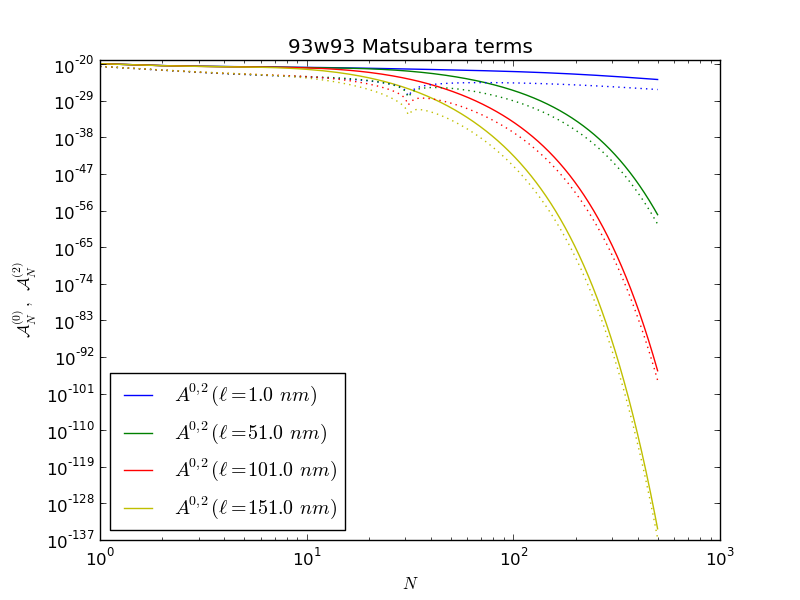
\includegraphics[width=1.0\textwidth]{plots/93_A_vs_n.png}
\hskip 43pt
\caption{Full result}
\label{eiz65}
\end{center}
\end{figure*} 

\subsection{[9,3] terms of modified Matsubara sum with $\mathcal{A}(n=0)=0$}
\begin{equation}
{\cal A}^{(0)}(\ell) = \frac{k_BT}{32}  {\sum_{n=0}^{\infty}}' \Delta_{1,\parallel} \Delta_{2,\parallel} ~p_n^{4}(\ell) ~\int_0^{\infty} t dt ~\frac{e^{- 2 p_n(\ell) \sqrt{t^{2} + 1}}}{(t^{2} + 1)} \tilde g^{(0)}(t, a_1(i \omega_n), a_2(i \omega_n))
\end{equation}

with

\begin{equation}
\tilde g^{(0)}(t, a_1(i \omega_n), a_2(i \omega_n)) = 2 \left[ (1+3a_1)(1+3a_2) t^{4} + 2 (1+2a_1+2a_2+3a_1a_2) t^{2}  + 2(1+a_1)(1+a_2)\right]
\end{equation}

and

\begin{equation}
{\cal A}^{(2)}(\ell) = \frac{k_BT}{32}  {\sum_{n=0}^{\infty}}' \Delta_{1,\parallel} \Delta_{2,\parallel} ~p_n^{4}(\ell) ~\int_0^{\infty} t dt ~\frac{e^{- 2 p_n(\ell) \sqrt{t^{2} + 1}}}{(t^{2} + 1)} \tilde g^{(2)}(t, a_1(i \omega_n), a_2(i \omega_n), \theta)
\end{equation}

with

\begin{equation}
\tilde g^{(2)}(t, a_1(i \omega_n), a_2(i \omega_n), \theta) = (1-a_1)(1-a_2)(t^{2} + 2)^2
\label{befgqw}
\end{equation}

\begin{figure*}[t!]
\begin{center}
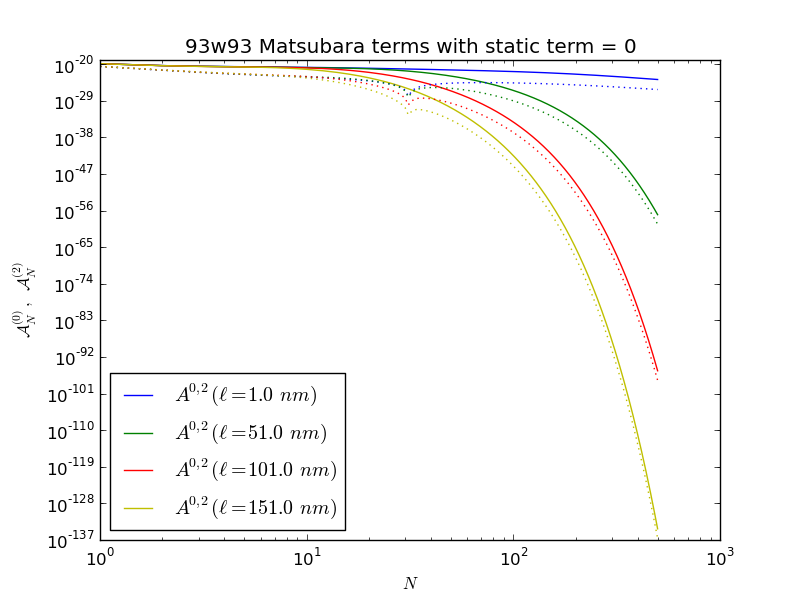
\includegraphics[width=1.0\textwidth]{plots/93_n0_A_vs_n.png}
\hskip 43pt
\caption{Full result}
\label{eiz65}
\end{center}
\end{figure*} 

%%%%%%%%%%%%%%%%%%%%%%%%%%%%%%%%% LOG A %%%%%%%%%%%%%%%%%%%%
\subsection{[9,3] Log-log plot of unmodified $\mathcal{A}$ }
\begin{equation}
{\cal A}^{(0)}(\ell) = \frac{k_BT}{32}  {\sum_{n=0}^{\infty}}' \Delta_{1,\parallel} \Delta_{2,\parallel} ~p_n^{4}(\ell) ~\int_0^{\infty} t dt ~\frac{e^{- 2 p_n(\ell) \sqrt{t^{2} + 1}}}{(t^{2} + 1)} \tilde g^{(0)}(t, a_1(i \omega_n), a_2(i \omega_n))
\end{equation}

with
\begin{multline*}
%\begin{equation}
%\begin{split}
\tilde g^{(0)}(t, a_1(i \omega_n), a_2(i \omega_n)) = \\ 
2 \left[ (1+3a_1)(1+3a_2) t^{4} + 2 (1+2a_1+2a_2+3a_1a_2) t^{2}  + 2(1+a_1)(1+a_2)\right]
%\end{split}
%\end{equation}
\end{multline*}


%\begin{equation}
%\tilde g^{(0)}(t, a_1(i \omega_n), a_2(i \omega_n)) = 2 \left[ (1+3a_1)(1+3a_2) t^{4} + 2 (1+2a_1+2a_2+3a_1a_2) t^{2}  + 2(1+a_1)(1+a_2)\right]
%\end{equation}

and

\begin{equation}
{\cal A}^{(2)}(\ell) = \frac{k_BT}{32}  {\sum_{n=0}^{\infty}}' \Delta_{1,\parallel} \Delta_{2,\parallel} ~p_n^{4}(\ell) ~\int_0^{\infty} t dt ~\frac{e^{- 2 p_n(\ell) \sqrt{t^{2} + 1}}}{(t^{2} + 1)} \tilde g^{(2)}(t, a_1(i \omega_n), a_2(i \omega_n), \theta)
\end{equation}

with

\begin{equation}
\tilde g^{(2)}(t, a_1(i \omega_n), a_2(i \omega_n), \theta) = (1-a_1)(1-a_2)(t^{2} + 2)^2
\label{befgqw}
\end{equation}

\begin{figure*}[t!]
\begin{center}
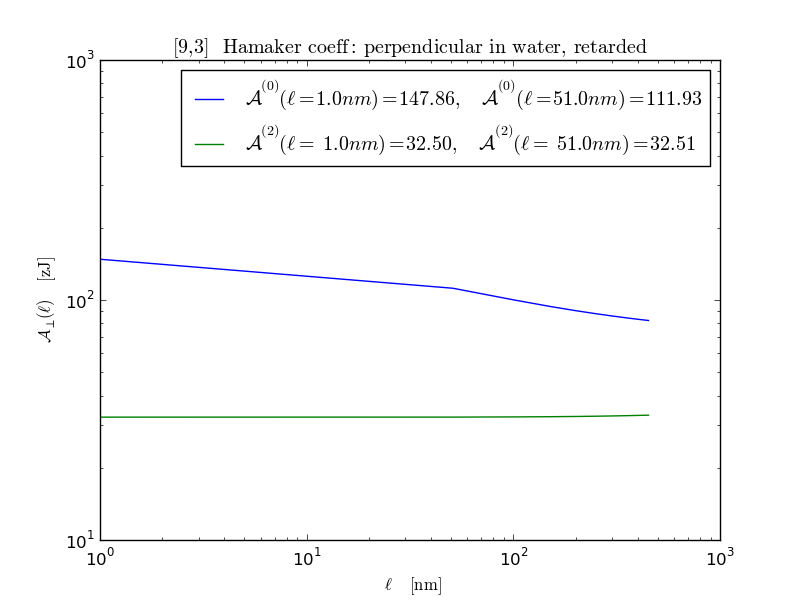
\includegraphics[width=1.0\textwidth]{plots/140322_93w93_HCs_perpendicular_ret.png}
\hskip 43pt
\caption{Full result}
\label{eiz65}
\end{center}
\end{figure*} 

\subsection{[9,3] Log-log plot of modified $\mathcal{A}(n=0)=0$}
\begin{equation}
{\cal A}^{(0)}(\ell) = \frac{k_BT}{32}  {\sum_{n=0}^{\infty}}' \Delta_{1,\parallel} \Delta_{2,\parallel} ~p_n^{4}(\ell) ~\int_0^{\infty} t dt ~\frac{e^{- 2 p_n(\ell) \sqrt{t^{2} + 1}}}{(t^{2} + 1)} \tilde g^{(0)}(t, a_1(i \omega_n), a_2(i \omega_n))
\end{equation}

with
\begin{multline*}
%\begin{equation}
%\begin{split}
\tilde g^{(0)}(t, a_1(i \omega_n), a_2(i \omega_n)) = \\ 
2 \left[ (1+3a_1)(1+3a_2) t^{4} + 2 (1+2a_1+2a_2+3a_1a_2) t^{2}  + 2(1+a_1)(1+a_2)\right]
%\end{split}
%\end{equation}
\end{multline*}


%\begin{equation}
%\tilde g^{(0)}(t, a_1(i \omega_n), a_2(i \omega_n)) = 2 \left[ (1+3a_1)(1+3a_2) t^{4} + 2 (1+2a_1+2a_2+3a_1a_2) t^{2}  + 2(1+a_1)(1+a_2)\right]
%\end{equation}

and

\begin{equation}
{\cal A}^{(2)}(\ell) = \frac{k_BT}{32}  {\sum_{n=0}^{\infty}}' \Delta_{1,\parallel} \Delta_{2,\parallel} ~p_n^{4}(\ell) ~\int_0^{\infty} t dt ~\frac{e^{- 2 p_n(\ell) \sqrt{t^{2} + 1}}}{(t^{2} + 1)} \tilde g^{(2)}(t, a_1(i \omega_n), a_2(i \omega_n), \theta)
\end{equation}

with

\begin{equation}
\tilde g^{(2)}(t, a_1(i \omega_n), a_2(i \omega_n), \theta) = (1-a_1)(1-a_2)(t^{2} + 2)^2
\label{befgqw}
\end{equation}

\begin{figure*}[t!]
\begin{center}
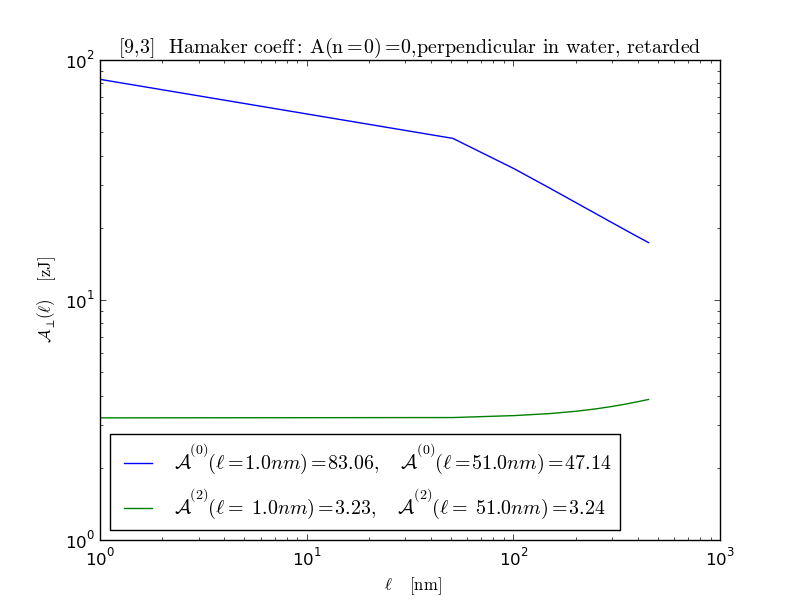
\includegraphics[width=1.0\textwidth]{plots/140322_93w93_HCs_n0_perpendicular_ret.png}
\hskip 43pt
\caption{Full result}
\label{eiz65}
\end{center}
\end{figure*}

%%%%%%%%%%%%%%%%%%%%%%%%%%%%%%%%% SEMILOG A %%%%%%%%%%%%%%%%
\subsection{[9,3] Semi-log plot of unmodified $\mathcal{A}$ }
\begin{equation}
{\cal A}^{(0)}(\ell) = \frac{k_BT}{32}  {\sum_{n=0}^{\infty}}' \Delta_{1,\parallel} \Delta_{2,\parallel} ~p_n^{4}(\ell) ~\int_0^{\infty} t dt ~\frac{e^{- 2 p_n(\ell) \sqrt{t^{2} + 1}}}{(t^{2} + 1)} \tilde g^{(0)}(t, a_1(i \omega_n), a_2(i \omega_n))
\end{equation}

with

\begin{multline*}
%\begin{equation}
%\begin{split}
\tilde g^{(0)}(t, a_1(i \omega_n), a_2(i \omega_n)) = \\ 
2 \left[ (1+3a_1)(1+3a_2) t^{4} + 2 (1+2a_1+2a_2+3a_1a_2) t^{2}  + 2(1+a_1)(1+a_2)\right]
%\end{split}
%\end{equation}
\end{multline*}

%\begin{equation}
%\tilde g^{(0)}(t, a_1(i \omega_n), a_2(i \omega_n)) = 2 \left[ (1+3a_1)(1+3a_2) t^{4} + 2 (1+2a_1+2a_2+3a_1a_2) t^{2}  + 2(1+a_1)(1+a_2)\right]
%\end{equation}

and

\begin{equation}
{\cal A}^{(2)}(\ell) = \frac{k_BT}{32}  {\sum_{n=0}^{\infty}}' \Delta_{1,\parallel} \Delta_{2,\parallel} ~p_n^{4}(\ell) ~\int_0^{\infty} t dt ~\frac{e^{- 2 p_n(\ell) \sqrt{t^{2} + 1}}}{(t^{2} + 1)} \tilde g^{(2)}(t, a_1(i \omega_n), a_2(i \omega_n), \theta)
\end{equation}

with

\begin{equation}
\tilde g^{(2)}(t, a_1(i \omega_n), a_2(i \omega_n), \theta) = (1-a_1)(1-a_2)(t^{2} + 2)^2
\label{befgqw}
\end{equation}

\begin{figure*}[t!]
\begin{center}
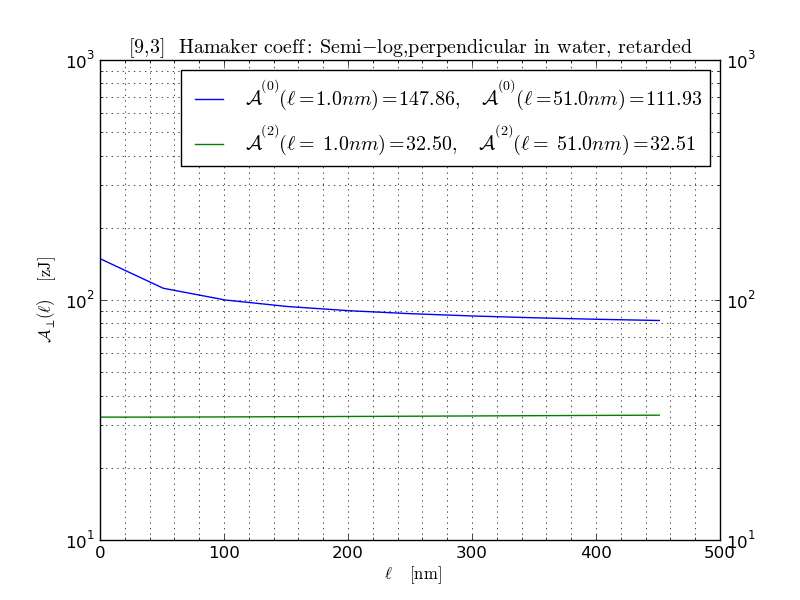
\includegraphics[width=1.0\textwidth]{plots/140322_93w93_HCs_semilog_perpendicular_ret.png}
\hskip 43pt
\caption{Full result}
\label{eiz65}
\end{center}
\end{figure*} 

\subsection{[9,3] Semi-log plot of modified $\mathcal{A}(n=0)=0$}
\begin{equation}
{\cal A}^{(0)}(\ell) = \frac{k_BT}{32}  {\sum_{n=0}^{\infty}}' \Delta_{1,\parallel} \Delta_{2,\parallel} ~p_n^{4}(\ell) ~\int_0^{\infty} t dt ~\frac{e^{- 2 p_n(\ell) \sqrt{t^{2} + 1}}}{(t^{2} + 1)} \tilde g^{(0)}(t, a_1(i \omega_n), a_2(i \omega_n))
\end{equation}

with

\begin{multline*}
%\begin{equation}
%\begin{split}
\tilde g^{(0)}(t, a_1(i \omega_n), a_2(i \omega_n)) = \\ 
2 \left[ (1+3a_1)(1+3a_2) t^{4} + 2 (1+2a_1+2a_2+3a_1a_2) t^{2}  + 2(1+a_1)(1+a_2)\right]
%\end{split}
%\end{equation}
\end{multline*}

%\begin{equation}
%\tilde g^{(0)}(t, a_1(i \omega_n), a_2(i \omega_n)) = 2 \left[ (1+3a_1)(1+3a_2) t^{4} + 2 (1+2a_1+2a_2+3a_1a_2) t^{2}  + 2(1+a_1)(1+a_2)\right]
%\end{equation}
%
and

\begin{equation}
{\cal A}^{(2)}(\ell) = \frac{k_BT}{32}  {\sum_{n=0}^{\infty}}' \Delta_{1,\parallel} \Delta_{2,\parallel} ~p_n^{4}(\ell) ~\int_0^{\infty} t dt ~\frac{e^{- 2 p_n(\ell) \sqrt{t^{2} + 1}}}{(t^{2} + 1)} \tilde g^{(2)}(t, a_1(i \omega_n), a_2(i \omega_n), \theta)
\end{equation}

with

\begin{equation}
\tilde g^{(2)}(t, a_1(i \omega_n), a_2(i \omega_n), \theta) = (1-a_1)(1-a_2)(t^{2} + 2)^2
\label{befgqw}
\end{equation}

\begin{figure*}[t!]
\begin{center}
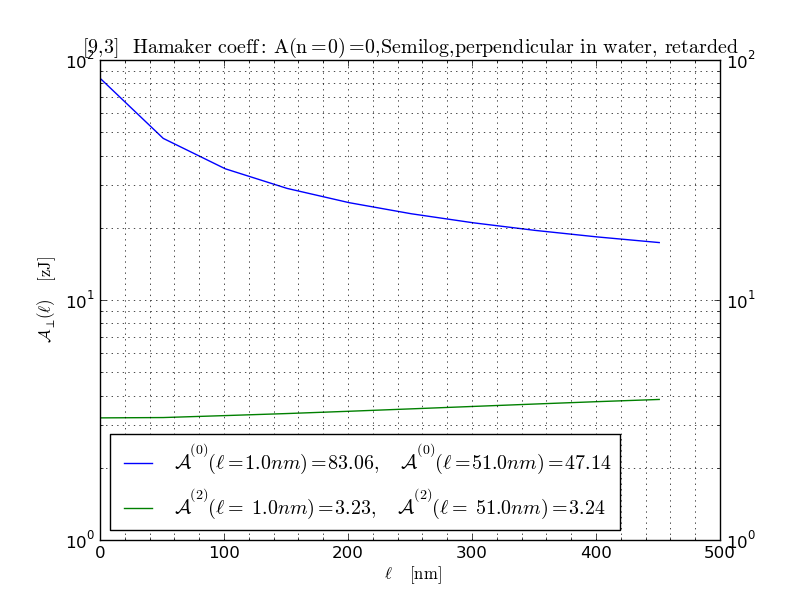
\includegraphics[width=1.0\textwidth]{plots/140322_93w93_HCs_n0_semilog_perpendicular_ret.png}
\hskip 43pt
\caption{Full result}
\label{eiz65}
\end{center}
\end{figure*} 

%%%%%%%%%%%%%%%%%%%%%%%%%%%%%%%%% [29,0] A %%%%%%%%%%%%%%%%%%%%%%%%%%%%%%%%%%%%%
\section{Semi-conductor [29,0]}
\subsection{[29,0] terms of Matsubara sum}
\begin{equation}
{\cal A}^{(0)}(\ell) = \frac{k_BT}{32}  {\sum_{n=0}^{\infty}}' \Delta_{1,\parallel} \Delta_{2,\parallel} ~p_n^{4}(\ell) ~\int_0^{\infty} t dt ~\frac{e^{- 2 p_n(\ell) \sqrt{t^{2} + 1}}}{(t^{2} + 1)} \tilde g^{(0)}(t, a_1(i \omega_n), a_2(i \omega_n))
\end{equation}

with

\begin{multline*}
%\begin{equation}
%\begin{split}
\tilde g^{(0)}(t, a_1(i \omega_n), a_2(i \omega_n)) = \\ 
2 \left[ (1+3a_1)(1+3a_2) t^{4} + 2 (1+2a_1+2a_2+3a_1a_2) t^{2}  + 2(1+a_1)(1+a_2)\right]
%\end{split}
%\end{equation}
\end{multline*}

%\begin{equation}
%\tilde g^{(0)}(t, a_1(i \omega_n), a_2(i \omega_n)) = 2 \left[ (1+3a_1)(1+3a_2) t^{4} + 2 (1+2a_1+2a_2+3a_1a_2) t^{2}  + 2(1+a_1)(1+a_2)\right]
%\end{equation}

and

\begin{equation}
{\cal A}^{(2)}(\ell) = \frac{k_BT}{32}  {\sum_{n=0}^{\infty}}' \Delta_{1,\parallel} \Delta_{2,\parallel} ~p_n^{4}(\ell) ~\int_0^{\infty} t dt ~\frac{e^{- 2 p_n(\ell) \sqrt{t^{2} + 1}}}{(t^{2} + 1)} \tilde g^{(2)}(t, a_1(i \omega_n), a_2(i \omega_n), \theta)
\end{equation}

with

\begin{equation}
\tilde g^{(2)}(t, a_1(i \omega_n), a_2(i \omega_n), \theta) = (1-a_1)(1-a_2)(t^{2} + 2)^2
\label{befgqw}
\end{equation}


\begin{figure*}[t!]
\begin{center}
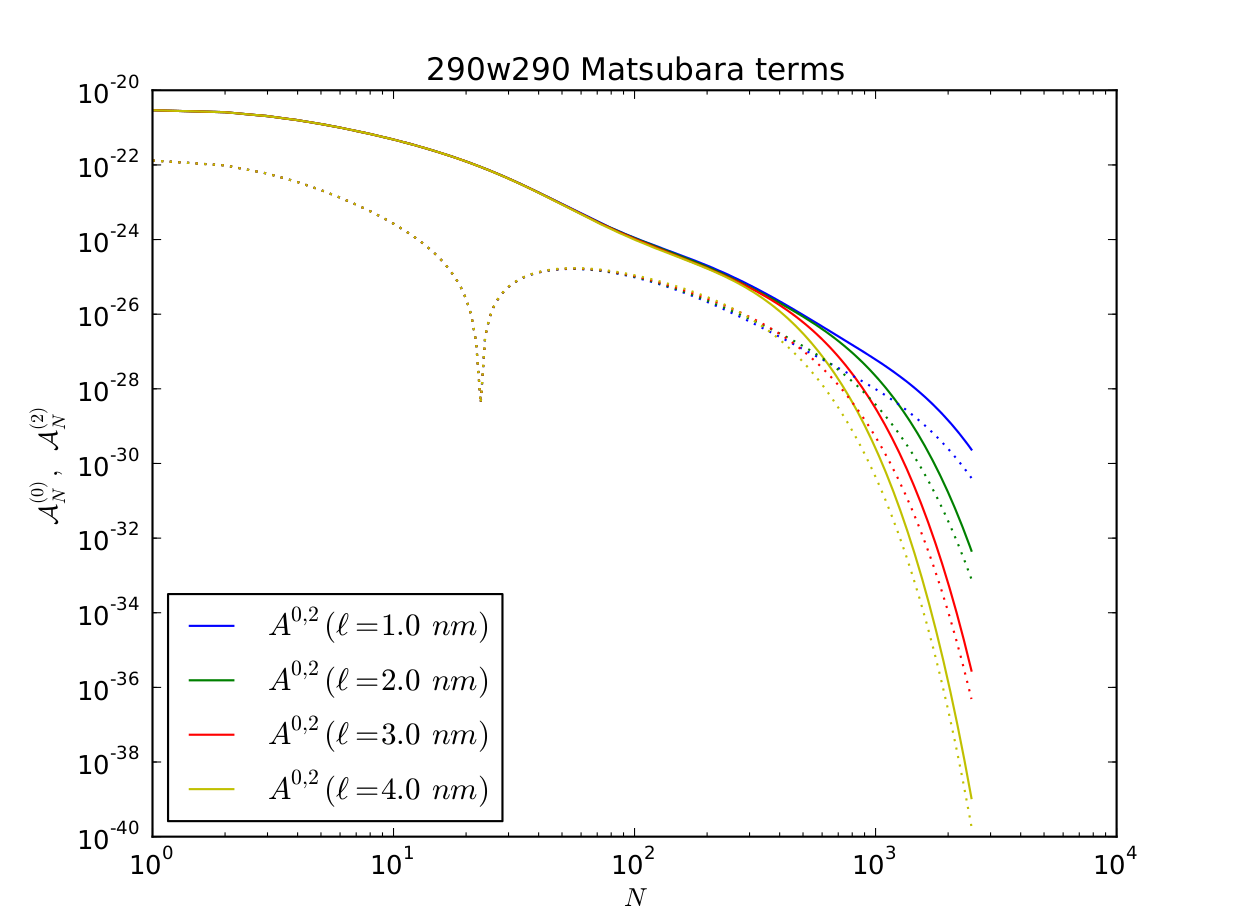
\includegraphics[width=1.2\textwidth]{large_N/290_A_vs_lrg_n.png}
\hskip 43pt
\caption{Full result}
\label{eiz65}
\end{center}
\end{figure*} 

%%%%%%%%%%%%%%%%%%%%%%%%%%%%%%%%% LOG A %%%%%%%%%%%%%%%%%%%%
\subsection{[29,0] Log-log plot of $\mathcal{A}^{(0)}$ and $\mathcal{A}^{(2)}$ }
\begin{equation}
{\cal A}^{(0)}(\ell) = \frac{k_BT}{32}  {\sum_{n=0}^{\infty}}' \Delta_{1,\parallel} \Delta_{2,\parallel} ~p_n^{4}(\ell) ~\int_0^{\infty} t dt ~\frac{e^{- 2 p_n(\ell) \sqrt{t^{2} + 1}}}{(t^{2} + 1)} \tilde g^{(0)}(t, a_1(i \omega_n), a_2(i \omega_n))
\end{equation}

with
\begin{multline*}
%\begin{equation}
%\begin{split}
\tilde g^{(0)}(t, a_1(i \omega_n), a_2(i \omega_n)) = \\ 
2 \left[ (1+3a_1)(1+3a_2) t^{4} + 2 (1+2a_1+2a_2+3a_1a_2) t^{2}  + 2(1+a_1)(1+a_2)\right]
%\end{split}
%\end{equation}
\end{multline*}


%\begin{equation}
%\tilde g^{(0)}(t, a_1(i \omega_n), a_2(i \omega_n)) = 2 \left[ (1+3a_1)(1+3a_2) t^{4} + 2 (1+2a_1+2a_2+3a_1a_2) t^{2}  + 2(1+a_1)(1+a_2)\right]
%\end{equation}
%
and

\begin{equation}
{\cal A}^{(2)}(\ell) = \frac{k_BT}{32}  {\sum_{n=0}^{\infty}}' \Delta_{1,\parallel} \Delta_{2,\parallel} ~p_n^{4}(\ell) ~\int_0^{\infty} t dt ~\frac{e^{- 2 p_n(\ell) \sqrt{t^{2} + 1}}}{(t^{2} + 1)} \tilde g^{(2)}(t, a_1(i \omega_n), a_2(i \omega_n), \theta)
\end{equation}

with

\begin{equation}
\tilde g^{(2)}(t, a_1(i \omega_n), a_2(i \omega_n), \theta) = (1-a_1)(1-a_2)(t^{2} + 2)^2
\label{befgqw}
\end{equation}

\begin{figure*}[t!]
\begin{center}
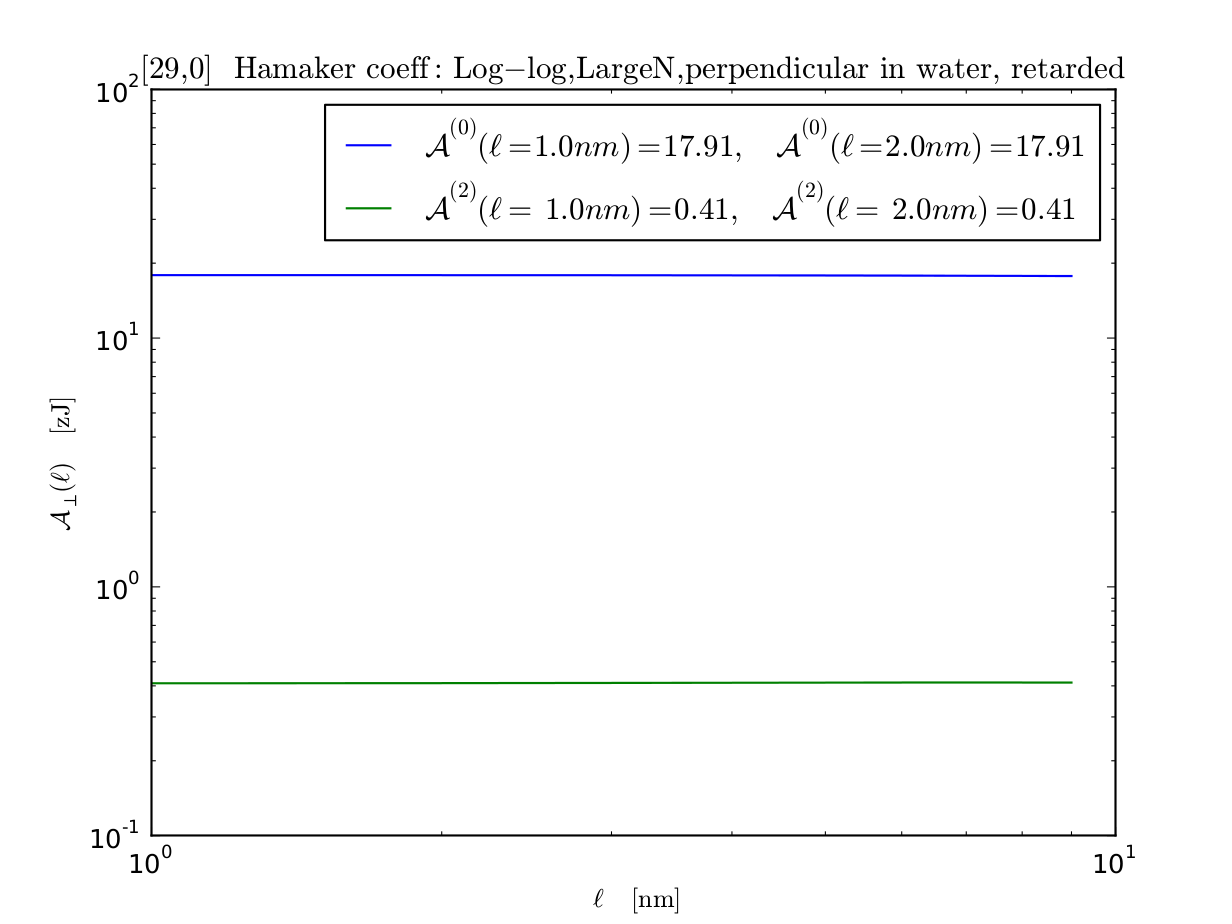
\includegraphics[width=1.2\textwidth]{large_N/140322_290w290_HCs_perpendicular_ret_lrg_n.png}
\hskip 43pt
\caption{Full result}
\label{eiz65}
\end{center}
\end{figure*} 

%%%%%%%%%%%%%%%%%%%%%%%%%%%%%%%%% SEMILOG A %%%%%%%%%%%%%%%%
\subsection{[29,0] Semi-log plot of $\mathcal{A}^{(0)}$ and $\mathcal{A}^{(2)}$ }
\begin{equation}
{\cal A}^{(0)}(\ell) = \frac{k_BT}{32}  {\sum_{n=0}^{\infty}}' \Delta_{1,\parallel} \Delta_{2,\parallel} ~p_n^{4}(\ell) ~\int_0^{\infty} t dt ~\frac{e^{- 2 p_n(\ell) \sqrt{t^{2} + 1}}}{(t^{2} + 1)} \tilde g^{(0)}(t, a_1(i \omega_n), a_2(i \omega_n))
\end{equation}

with

\begin{multline*}
%\begin{equation}
%\begin{split}
\tilde g^{(0)}(t, a_1(i \omega_n), a_2(i \omega_n)) = \\ 
2 \left[ (1+3a_1)(1+3a_2) t^{4} + 2 (1+2a_1+2a_2+3a_1a_2) t^{2}  + 2(1+a_1)(1+a_2)\right]
%\end{split}
%\end{equation}
\end{multline*}

%\begin{equation}
%\tilde g^{(0)}(t, a_1(i \omega_n), a_2(i \omega_n)) = 2 \left[ (1+3a_1)(1+3a_2) t^{4} + 2 (1+2a_1+2a_2+3a_1a_2) t^{2}  + 2(1+a_1)(1+a_2)\right]
%\end{equation}

and

\begin{equation}
{\cal A}^{(2)}(\ell) = \frac{k_BT}{32}  {\sum_{n=0}^{\infty}}' \Delta_{1,\parallel} \Delta_{2,\parallel} ~p_n^{4}(\ell) ~\int_0^{\infty} t dt ~\frac{e^{- 2 p_n(\ell) \sqrt{t^{2} + 1}}}{(t^{2} + 1)} \tilde g^{(2)}(t, a_1(i \omega_n), a_2(i \omega_n), \theta)
\end{equation}

with

\begin{equation}
\tilde g^{(2)}(t, a_1(i \omega_n), a_2(i \omega_n), \theta) = (1-a_1)(1-a_2)(t^{2} + 2)^2
\label{befgqw}
\end{equation}

\begin{figure*}[t!]
\begin{center}
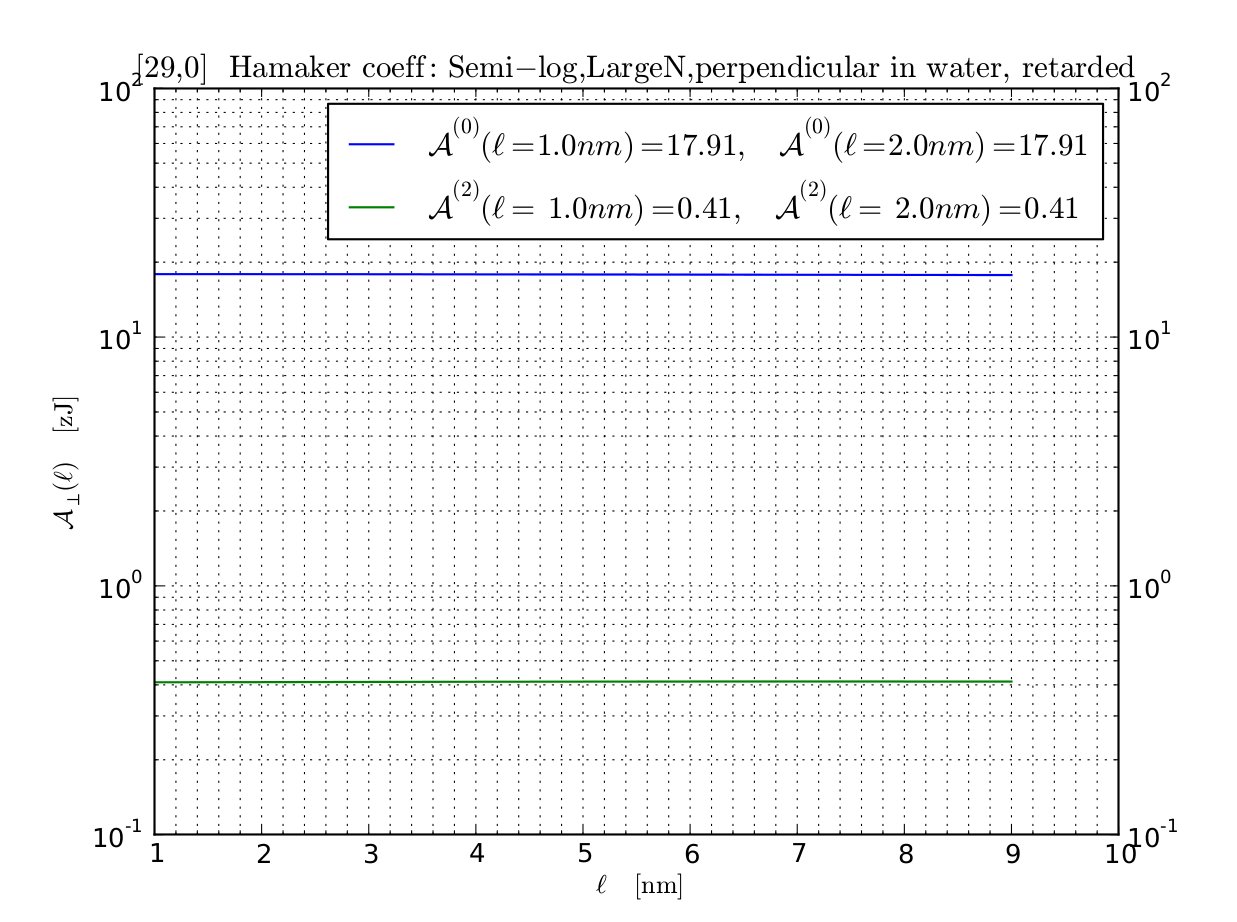
\includegraphics[width=1.2\textwidth]{large_N/140322_290w290_HCs_semilog_perpendicular_ret_lrg_n.png}
\hskip 43pt
\caption{Full result}
\label{eiz65}
\end{center}
\end{figure*} 

%%%%%%%%%%%%%%%%%%%%%%%%%%%%%%%%%A0 and A2 plot FOR KINK in [9,3] A0 %%%%%%%%%%%
\chapter{Knee in plots of $\mathcal{A}^{(0)}$ as a function of separation}

\section{An example plot of knee: $\mathcal{A}^{(0)}$ for [9,3]}
%\subsection{Plot of $\mathcal{A}^{(0)}$ and $\mathcal{A}^{(2)}$ for [9,3]}
\begin{equation}
{\cal A}^{(0)}(\ell) = \frac{k_BT}{32}  {\sum_{n=0}^{\infty}}' \Delta_{1,\parallel} \Delta_{2,\parallel} ~p_n^{4}(\ell) ~\int_0^{\infty} t dt ~\frac{e^{- 2 p_n(\ell) \sqrt{t^{2} + 1}}}{(t^{2} + 1)} \tilde g^{(0)}(t, a_1(i \omega_n), a_2(i \omega_n))
\end{equation}

with
\begin{multline*}
%\begin{equation}
%\begin{split}
\tilde g^{(0)}(t, a_1(i \omega_n), a_2(i \omega_n)) = \\ 
2 \left[ (1+3a_1)(1+3a_2) t^{4} + 2 (1+2a_1+2a_2+3a_1a_2) t^{2}  + 2(1+a_1)(1+a_2)\right]
%\end{split}
%\end{equation}
\end{multline*}


%\begin{equation}
%\tilde g^{(0)}(t, a_1(i \omega_n), a_2(i \omega_n)) = 2 \left[ (1+3a_1)(1+3a_2) t^{4} + 2 (1+2a_1+2a_2+3a_1a_2) t^{2}  + 2(1+a_1)(1+a_2)\right]
%\end{equation}

and

\begin{equation}
{\cal A}^{(2)}(\ell) = \frac{k_BT}{32}  {\sum_{n=0}^{\infty}}' \Delta_{1,\parallel} \Delta_{2,\parallel} ~p_n^{4}(\ell) ~\int_0^{\infty} t dt ~\frac{e^{- 2 p_n(\ell) \sqrt{t^{2} + 1}}}{(t^{2} + 1)} \tilde g^{(2)}(t, a_1(i \omega_n), a_2(i \omega_n), \theta)
\end{equation}

with

\begin{equation}
\tilde g^{(2)}(t, a_1(i \omega_n), a_2(i \omega_n), \theta) = (1-a_1)(1-a_2)(t^{2} + 2)^2
\label{befgqw}
\end{equation}

\begin{figure*}[t!]
\begin{center}
    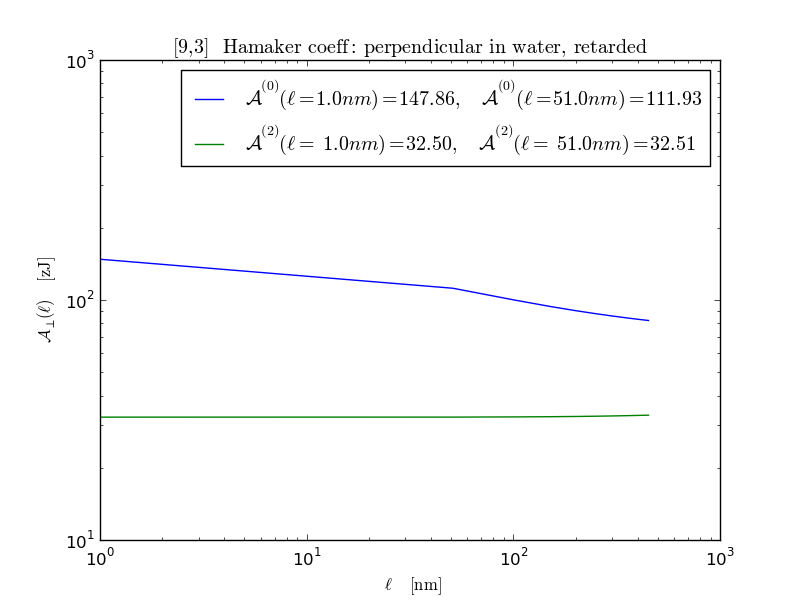
\includegraphics[width=1.2\textwidth]{plots/140322_93w93_HCs_perpendicular_ret.png}
\hskip 43pt
\caption{$\mathcal{A}^{(0)}$ as a function of separation appears to have a knee near 36 nm.}
\label{eiz65}
\end{center}
\end{figure*} 

%%%%%%%%%%%%%%%%%%%%%%%%%%%%PLOT OF p(n,l)%%%%%%%%%%%%%%%%%%
The $(\ell)$ dependence of the Hamaker coefficients $\cal A$ is a consequence of $(\ell)$ dependence of $p_n^{2}(\ell) =  \epsilon_m(i \omega_n) \frac{\omega_n^{2}}{c^{2}} \ell^{2}$

\begin{equation}
{\cal A}^{(0)}(\ell) = \frac{k_BT}{32}  {\sum_{n=0}^{\infty}}' \Delta_{1,\parallel} \Delta_{2,\parallel} ~p_n^{4}(\ell) ~\int_0^{\infty} t dt ~\frac{e^{- 2 p_n(\ell) \sqrt{t^{2} + 1}}}{(t^{2} + 1)} \tilde g^{(0)}(t, a_1(i \omega_n), a_2(i \omega_n))
\end{equation}

with

\begin{equation}
\tilde g^{(0)}(t, a_1(i \omega_n), a_2(i \omega_n)) = 2 \left[ (1+3a_1)(1+3a_2) t^{4} + 2 (1+2a_1+2a_2+3a_1a_2) t^{2}  + 2(1+a_1)(1+a_2)\right]
\end{equation}

and

\begin{equation}
{\cal A}^{(2)}(\ell) = \frac{k_BT}{32}  {\sum_{n=0}^{\infty}}' \Delta_{1,\parallel} \Delta_{2,\parallel} ~p_n^{4}(\ell) ~\int_0^{\infty} t dt ~\frac{e^{- 2 p_n(\ell) \sqrt{t^{2} + 1}}}{(t^{2} + 1)} \tilde g^{(2)}(t, a_1(i \omega_n), a_2(i \omega_n), \theta)
\end{equation}

with

\begin{equation}
\tilde g^{(2)}(t, a_1(i \omega_n), a_2(i \omega_n), \theta) = (1-a_1)(1-a_2)(t^{2} + 2)^2
\label{befgqw}
\end{equation}

$\zeta_n = 2\pi n k_BT/\hbar$, where $n$ is an integer and the $n=0$ term is counted with a weight $1/2$. 

where $p_n^{2}(\ell) =  \epsilon_m(i \omega_n) \frac{\omega_n^{2}}{c^{2}} \ell^{2}$. 


%\section{How each Matsubara term contributes to $\mathcal{A}_{n}^{(0)}(\ell)$}
%where $p_n^{2}(\ell) =  \epsilon_m(i \omega_n) \frac{\omega_n^{2}}{c^{2}} \ell^{2}$. 
%\begin{figure*}[t!]
%\begin{center}
%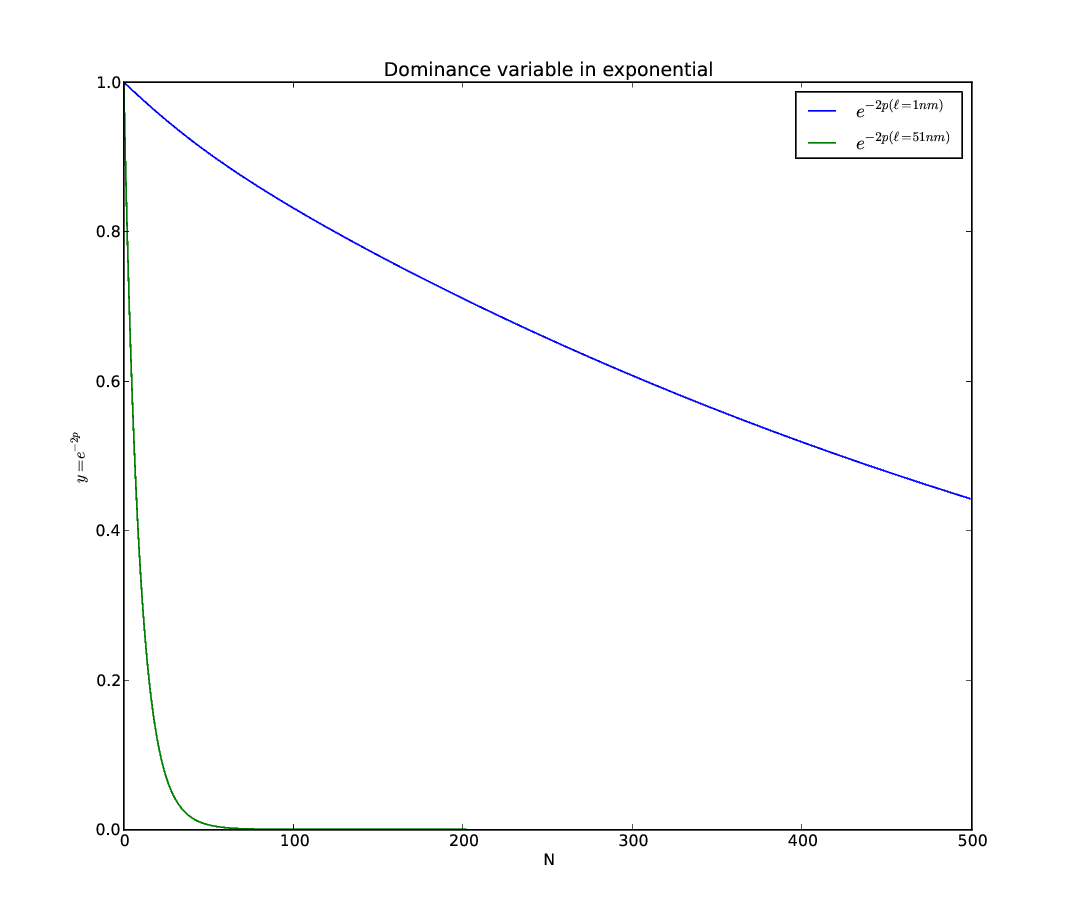
\includegraphics[width=1.2\textwidth]{plots/140415_93_n0_Dominance_variable_kink.png}
%\hskip 43pt
%\caption{The discontinuity in $\mathcal{A}^{(0)}$ at 36 nm separation is due to
%the change in dominating variable in the exponential.  Plot shows
%behavior of exponential term for separation values smaller (blue) and larger
%(green) than 36nm. At 1 nm, the exponential gives non-zero values. At 51 nm, the
%exponential is quickly dominated by $\ell$ and tends to zero.}
%\label{eiz65}
%\end{center}
%\end{figure*} 

\section{Plots of how each Matsubara term contributes to $\mathcal{A}_{n}^{(0)}(\ell)$}
%\subsection{Derivatives of Matsubara terms for $\mathcal{A}^{(0)}$ with respect
%to separation and n}
\begin{figure*}[t!]
\begin{center}
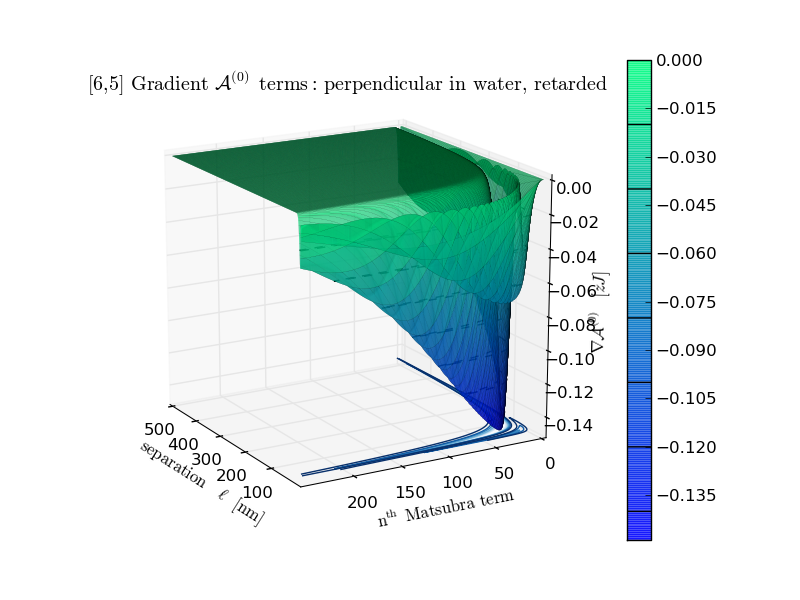
\includegraphics[width=1.4\textwidth]{plots/grad_A0_65.png}
\hskip 43pt
\caption{$\nabla(\mathcal{A}_{n}^{(0)}(\ell))$ for [6,5]: derivative of
$\mathcal{A}_{n}^{(0)}(\ell)$ (z-axis) with respect to separation and n (x and
y axes. $Max[\lvert \nabla(\mathcal{A}^{(0)}) \rvert]$ occurs at
$\ell=\ell_{knee}$}
\label{eiz65}
\end{center}
\end{figure*} 

\begin{figure*}[t!]
\begin{center}
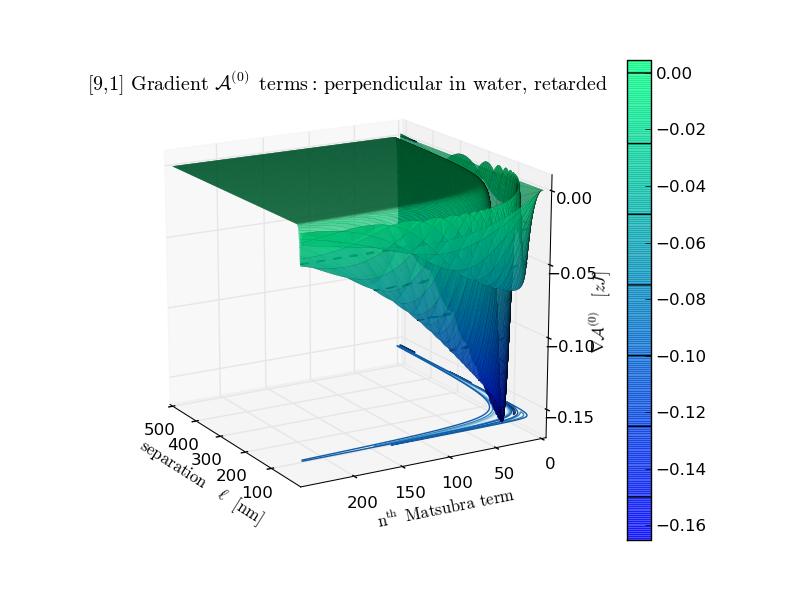
\includegraphics[width=1.4\textwidth]{plots/grad_A0_91.png}
\hskip 43pt
\caption{$\nabla(\mathcal{A}_{n}^{(0)}(\ell))$ for [9,1]: derivative of
$\mathcal{A}_{n}^{(0)}(\ell)$ (z-axis) with respect to separation and n (x and
y axes. $Max[\lvert \nabla(\mathcal{A}^{(0)}) \rvert]$ occurs at
$\ell=\ell_{knee}$}
\label{eiz65}
\end{center}
\end{figure*} 

\begin{figure*}[t!]
\begin{center}
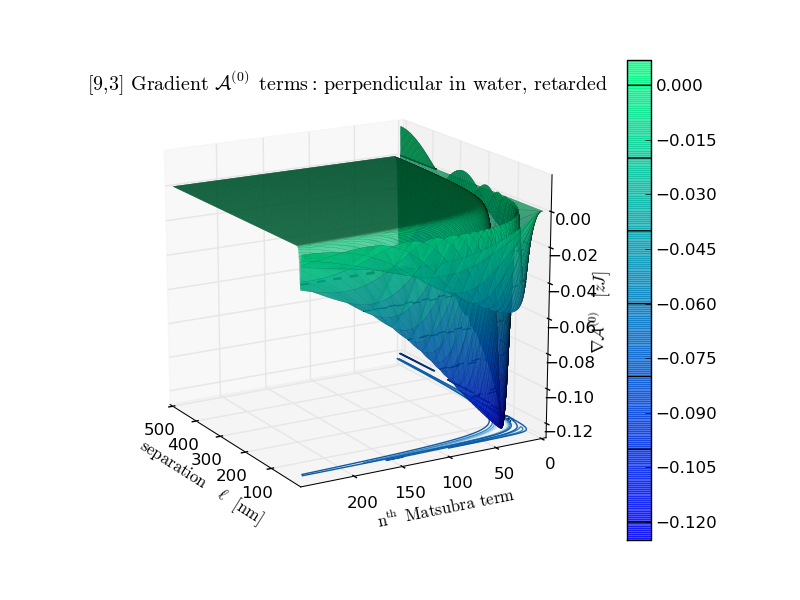
\includegraphics[width=1.4\textwidth]{plots/grad_A0_93.png}
\hskip 43pt
\caption{$\nabla(\mathcal{A}_{n}^{(0)}(\ell))$ for [9,3]: derivative of
$\mathcal{A}_{n}^{(0)}(\ell)$ (z-axis) with respect to separation and n (x and
y axes. $Max[\lvert \nabla(\mathcal{A}^{(0)}) \rvert]$ occurs at
$\ell=\ell_{knee}$}
\label{eiz65}
\end{center}
\end{figure*} 

\begin{figure*}[t!]
\begin{center}
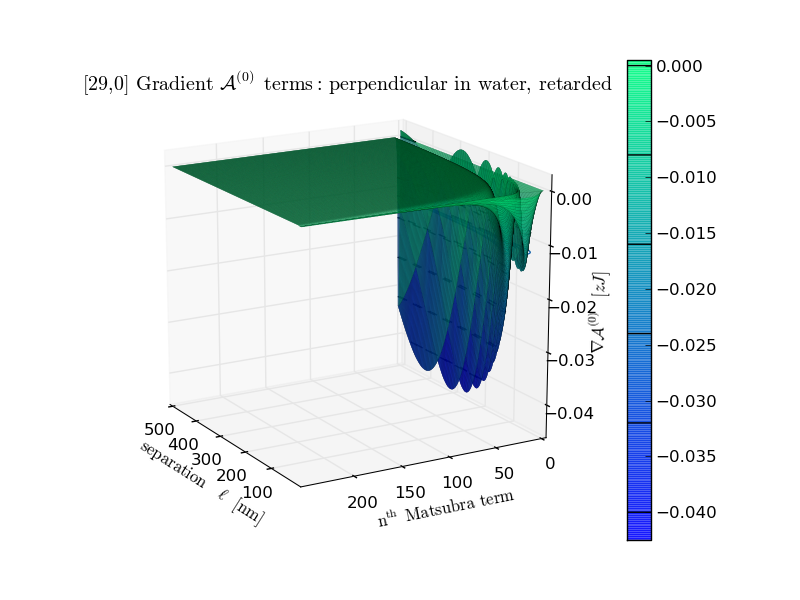
\includegraphics[width=1.4\textwidth]{plots/grad_A0_290.png}
\hskip 43pt
\caption{$\nabla(\mathcal{A}_{n}^{(0)}(\ell))$ for [29,0]: derivative of
$\mathcal{A}_{n}^{(0)}(\ell)$ (z-axis) with respect to separation and n (x and
y axes. $Max[\lvert \nabla(\mathcal{A}^{(0)}) \rvert]$ occurs at
$\ell=\ell_{knee}$}
\label{eiz65}
\end{center}
\end{figure*} 


\subsection{Plots for visualizing and comparing gradiants for different CNT's}% $\mathcal{A}_{n}^{(0)}(\ell)$}
\begin{figure*}[t!]
\begin{center}
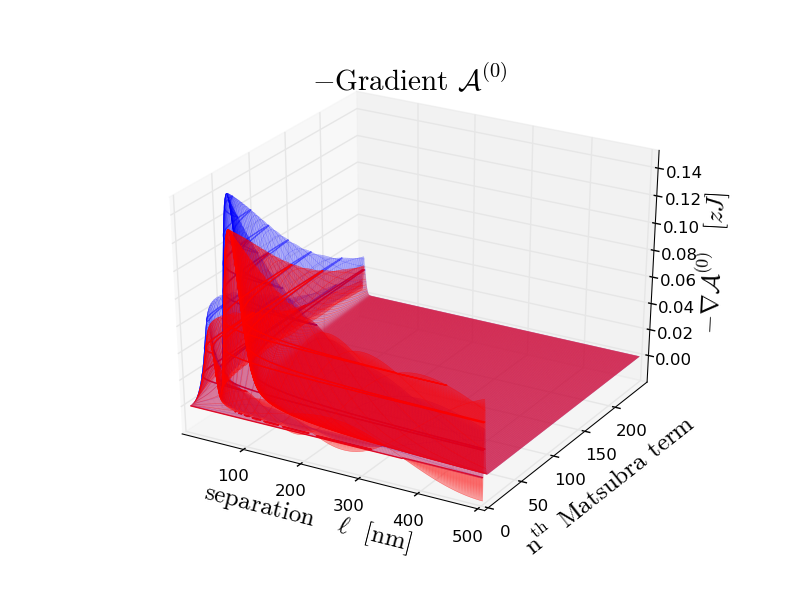
\includegraphics[width=1.2\textwidth]{plots/A0_wire2_0.png}
\hskip 43pt
\caption{$-\nabla(\mathcal{A}_{n}^{(0)}(\ell))$ for [6,5] (blue) and [9,3] (red)}
\label{eiz65}
\end{center}
\end{figure*} 

\begin{figure*}[t!]
\begin{center}
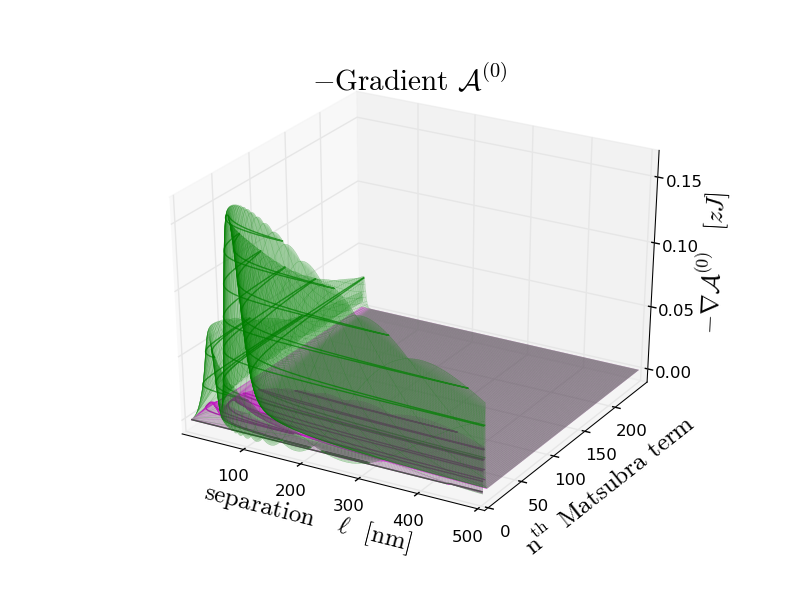
\includegraphics[width=1.2\textwidth]{plots/A0_wire2_1.png}
\hskip 43pt
\caption{$-\nabla(\mathcal{A}_{n}^{(0)}(\ell))$ for [9,1] (green) and [29,0]
(magenta)}
\label{eiz65}
\end{center}
\end{figure*} 

\begin{figure*}[t!]
\begin{center}
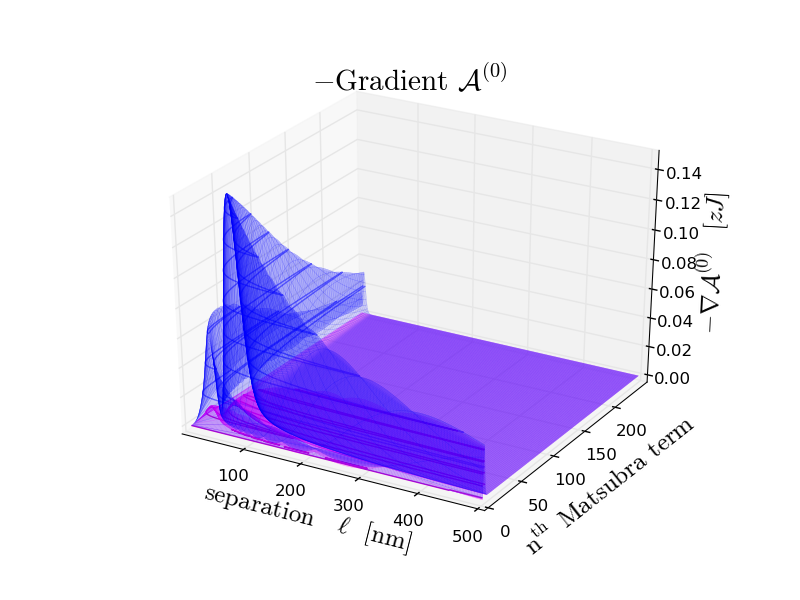
\includegraphics[width=1.2\textwidth]{plots/A0_wire2_2.png}
\hskip 43pt
\caption{$-\nabla(\mathcal{A}_{n}^{(0)}(\ell))$ for [6,5] (blue) and [29,0]
(magenta)}
%\caption{$\mathcal{A}^{(0)}$}
\label{eiz65}
\end{center}
\end{figure*} 

\begin{figure*}[t!]
\begin{center}
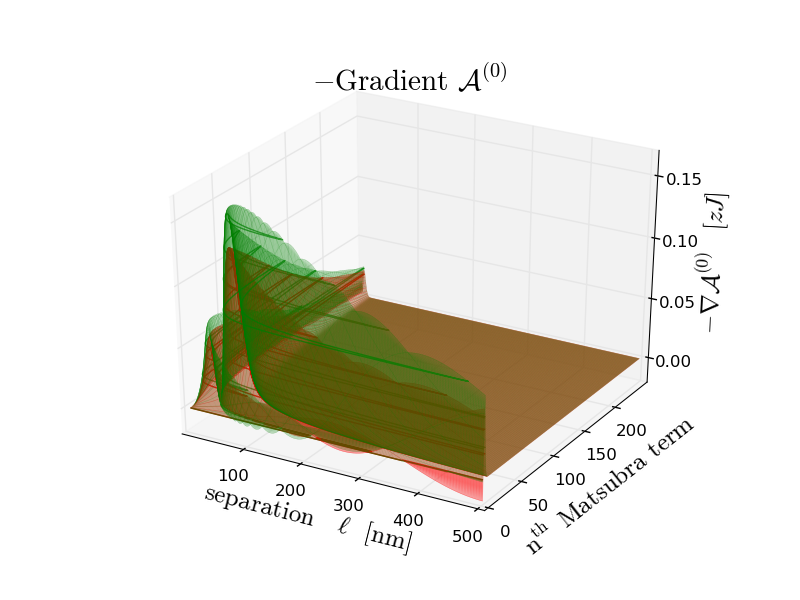
\includegraphics[width=1.2\textwidth]{plots/A0_wire2_3.png}
\hskip 43pt
\caption{$-\nabla(\mathcal{A}_{n}^{(0)}(\ell))$ for [9,1] (red) and [9,3] (green)}
\label{eiz65}
\end{center}
\end{figure*} 


%\chapter{Non-retarded Hamaker Coefficients}
%
%\section{[6,5]}
%\subsection{[6,5] terms of Matsubara sum}
%
%\section{[9,1] Non-retarded}
%\section{[29,0]}
%Here is the second paragraph\footnote{with a footnote}. 
%As you can see it's a rather short paragraph, but not 
%as short as the previous one. This document was 
%created on: \today\ at \currenttime.
%\subsection{[29,0] terms of Matsubara sum}
%This is a simple \LaTeX\ document.
%Here is the first paragraph.
%\subsection{[29,0] Log-log plot of $\mathcal{A}^{(0)}$ and $\mathcal{A}^{(2)}$ }
%This is a simple \LaTeX\ document.
%Here is the first paragraph.
%\subsection{[29,0] Semi-log plot of $\mathcal{A}^{(0)}$ and $\mathcal{A}^{(2)}$ }
%This is a simple \LaTeX\ document.
%Here is the first paragraph.

%%%%%%%%%%%%%% COMBO SURFACE PLOTs %%%%%%%%%%%%%%%%%%%%%%%%%%%%%%%%%%%%%%%%%%%%%
\chapter{Surface plots for Hamaker Coefficients as function of angle and
separation}

\section{Fully Retarded}

\subsection{$\mathcal{A}^{(0)}$ for [6,5], [9,1], and [29,0] in water}
%%%%%%%%%%%%%% A0 COMBO SURF PLOT %%%%%%%%%%%%%%%%%%%%%%%%%%
\begin{equation}
{\cal A}^{(0)}(\ell) = \frac{k_BT}{32}  {\sum_{n=0}^{\infty}}' \Delta_{1,\parallel} \Delta_{2,\parallel} ~p_n^{4}(\ell) ~\int_0^{\infty} t dt ~\frac{e^{- 2 p_n(\ell) \sqrt{t^{2} + 1}}}{(t^{2} + 1)} \tilde g^{(0)}(t, a_1(i \omega_n), a_2(i \omega_n))
\end{equation}

with

\begin{equation}
\tilde g^{(0)}(t, a_1(i \omega_n), a_2(i \omega_n)) = 2 \left[ (1+3a_1)(1+3a_2) t^{4} + 2 (1+2a_1+2a_2+3a_1a_2) t^{2}  + 2(1+a_1)(1+a_2)\right]
\end{equation}

and

\begin{equation}
{\cal A}^{(2)}(\ell) = \frac{k_BT}{32}  {\sum_{n=0}^{\infty}}' \Delta_{1,\parallel} \Delta_{2,\parallel} ~p_n^{4}(\ell) ~\int_0^{\infty} t dt ~\frac{e^{- 2 p_n(\ell) \sqrt{t^{2} + 1}}}{(t^{2} + 1)} \tilde g^{(2)}(t, a_1(i \omega_n), a_2(i \omega_n), \theta)
\end{equation}

with

\begin{equation}
\tilde g^{(2)}(t, a_1(i \omega_n), a_2(i \omega_n), \theta) = (1-a_1)(1-a_2)(t^{2} + 2)^2
\label{befgqw}
\end{equation}

\begin{figure*}[t!]
\begin{center}
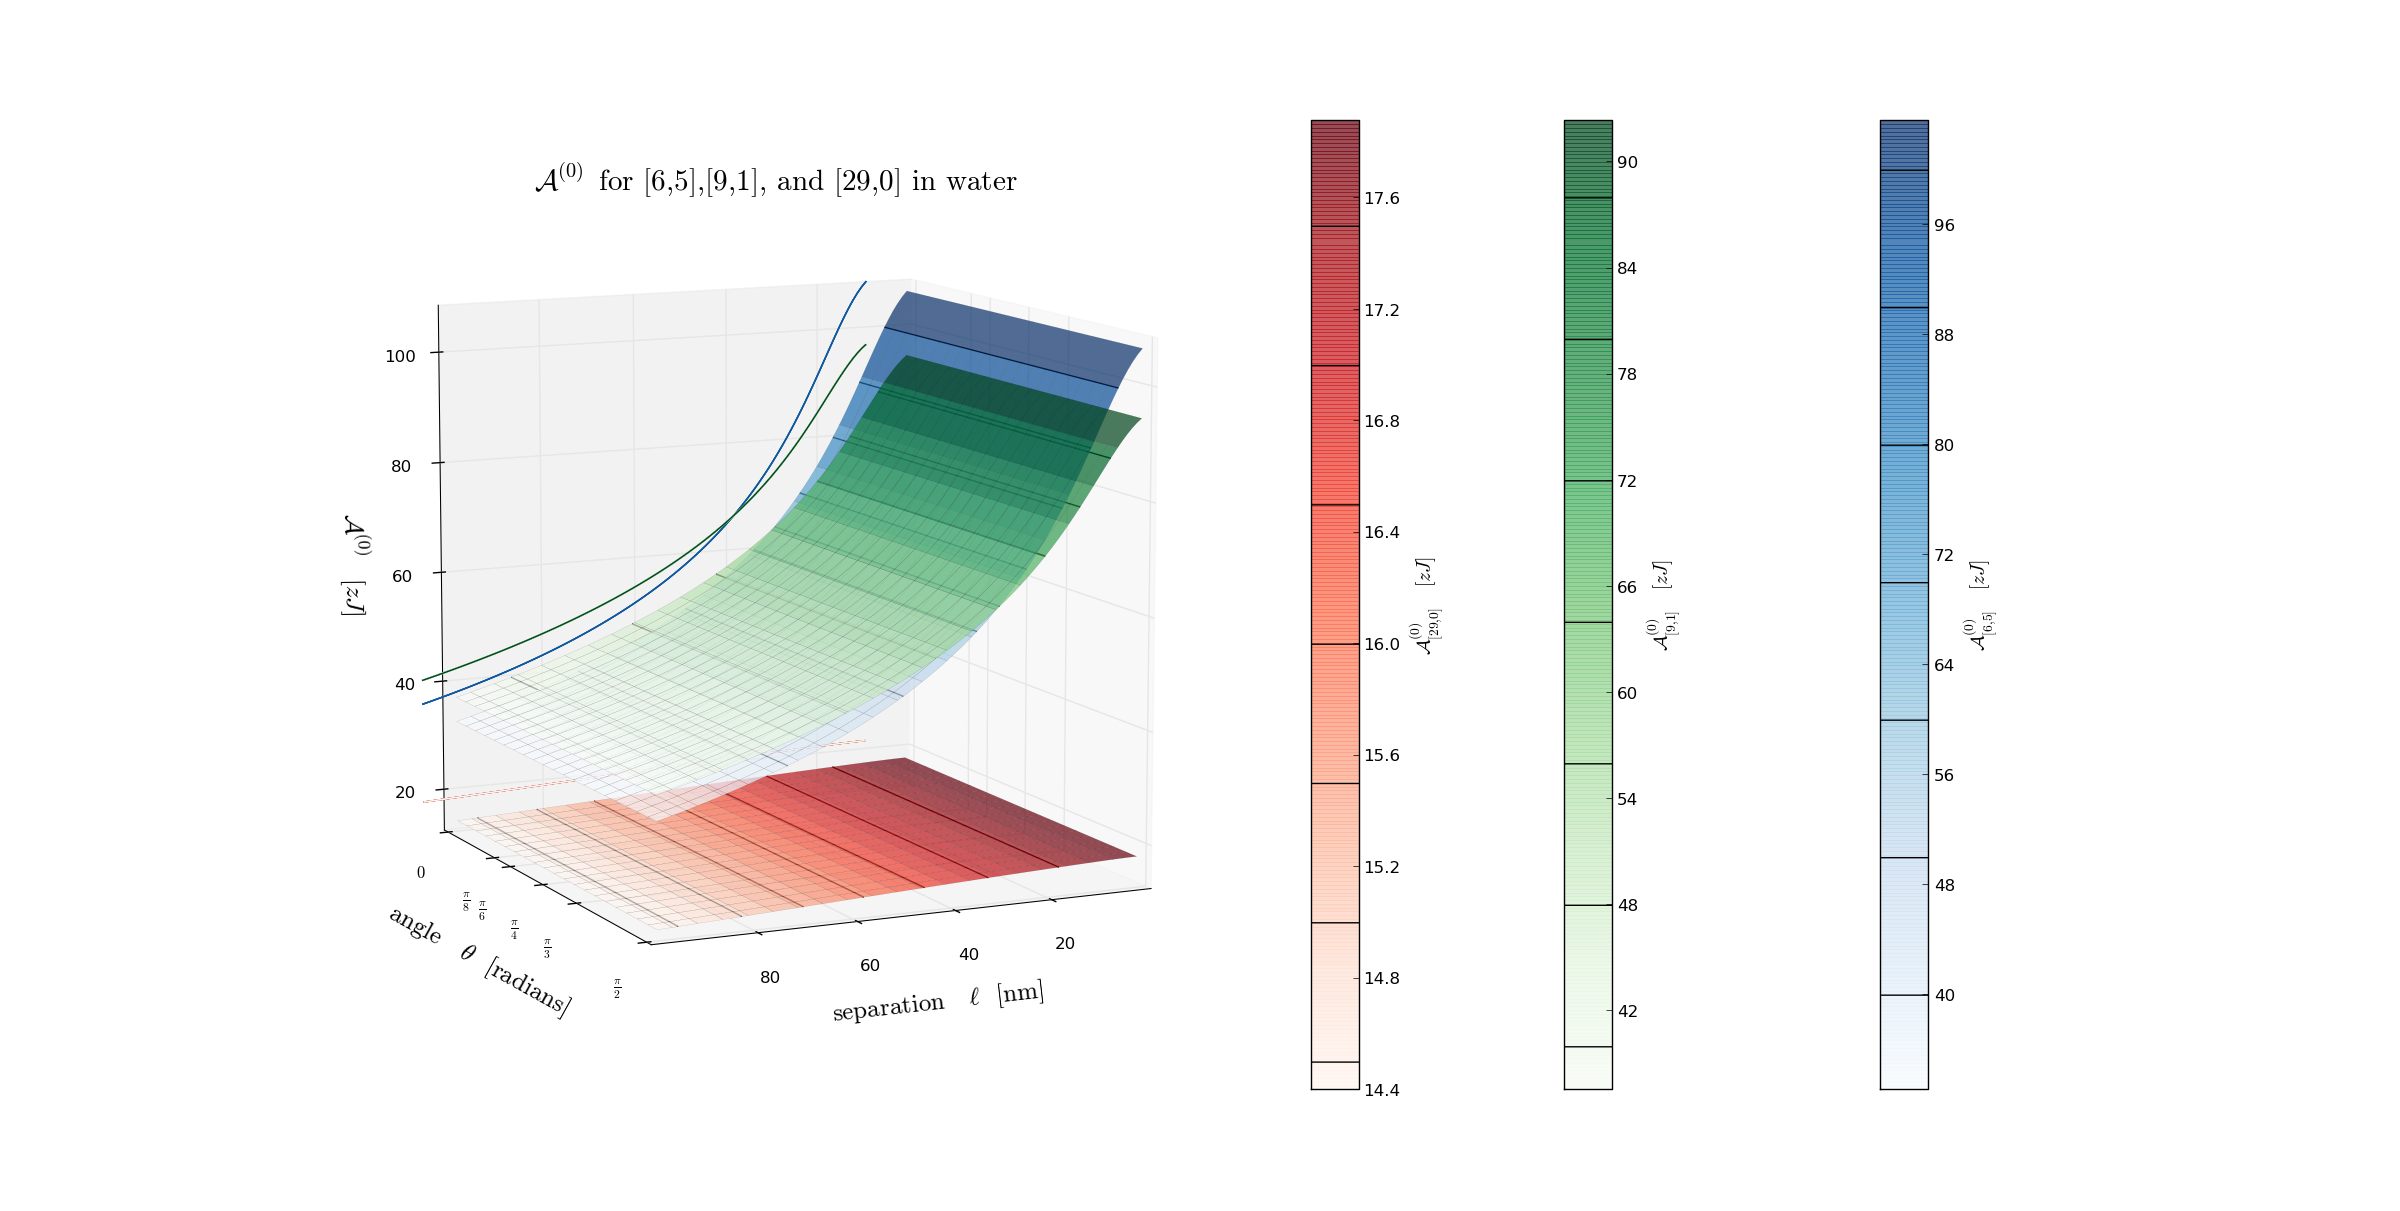
\includegraphics[width=1.5\textwidth]{plots/A0_65_91_290_srw.png}
\hskip 43pt
\caption{$\mathcal{A}^{(0)}$ for [6,5], [9,1], and [29,0] in water. No theta
dependence}
\label{eiz65}
\end{center}
\end{figure*} 

\subsection{Hamaker 2: $\mathcal{A}^{(2)}$ for [6,5], [9,1], and [29,0] in water }
%%%%%%%%%A2 COMBO SURF PLOT%%%%%%%%%%%%%%%%%%%%%%%%%%%%%%%%%
\begin{equation}
{\cal A}^{(0)}(\ell) = \frac{k_BT}{32}  {\sum_{n=0}^{\infty}}' \Delta_{1,\parallel} \Delta_{2,\parallel} ~p_n^{4}(\ell) ~\int_0^{\infty} t dt ~\frac{e^{- 2 p_n(\ell) \sqrt{t^{2} + 1}}}{(t^{2} + 1)} \tilde g^{(0)}(t, a_1(i \omega_n), a_2(i \omega_n))
\end{equation}

with

\begin{equation}
\tilde g^{(0)}(t, a_1(i \omega_n), a_2(i \omega_n)) = 2 \left[ (1+3a_1)(1+3a_2) t^{4} + 2 (1+2a_1+2a_2+3a_1a_2) t^{2}  + 2(1+a_1)(1+a_2)\right]
\end{equation}

and

\begin{equation}
{\cal A}^{(2)}(\ell) = \frac{k_BT}{32}  {\sum_{n=0}^{\infty}}' \Delta_{1,\parallel} \Delta_{2,\parallel} ~p_n^{4}(\ell) ~\int_0^{\infty} t dt ~\frac{e^{- 2 p_n(\ell) \sqrt{t^{2} + 1}}}{(t^{2} + 1)} \tilde g^{(2)}(t, a_1(i \omega_n), a_2(i \omega_n), \theta)
\end{equation}

with

\begin{equation}
\tilde g^{(2)}(t, a_1(i \omega_n), a_2(i \omega_n), \theta) = (1-a_1)(1-a_2)(t^{2} + 2)^2
\label{befgqw}
\end{equation}

\begin{figure*}[t!]
\begin{center}
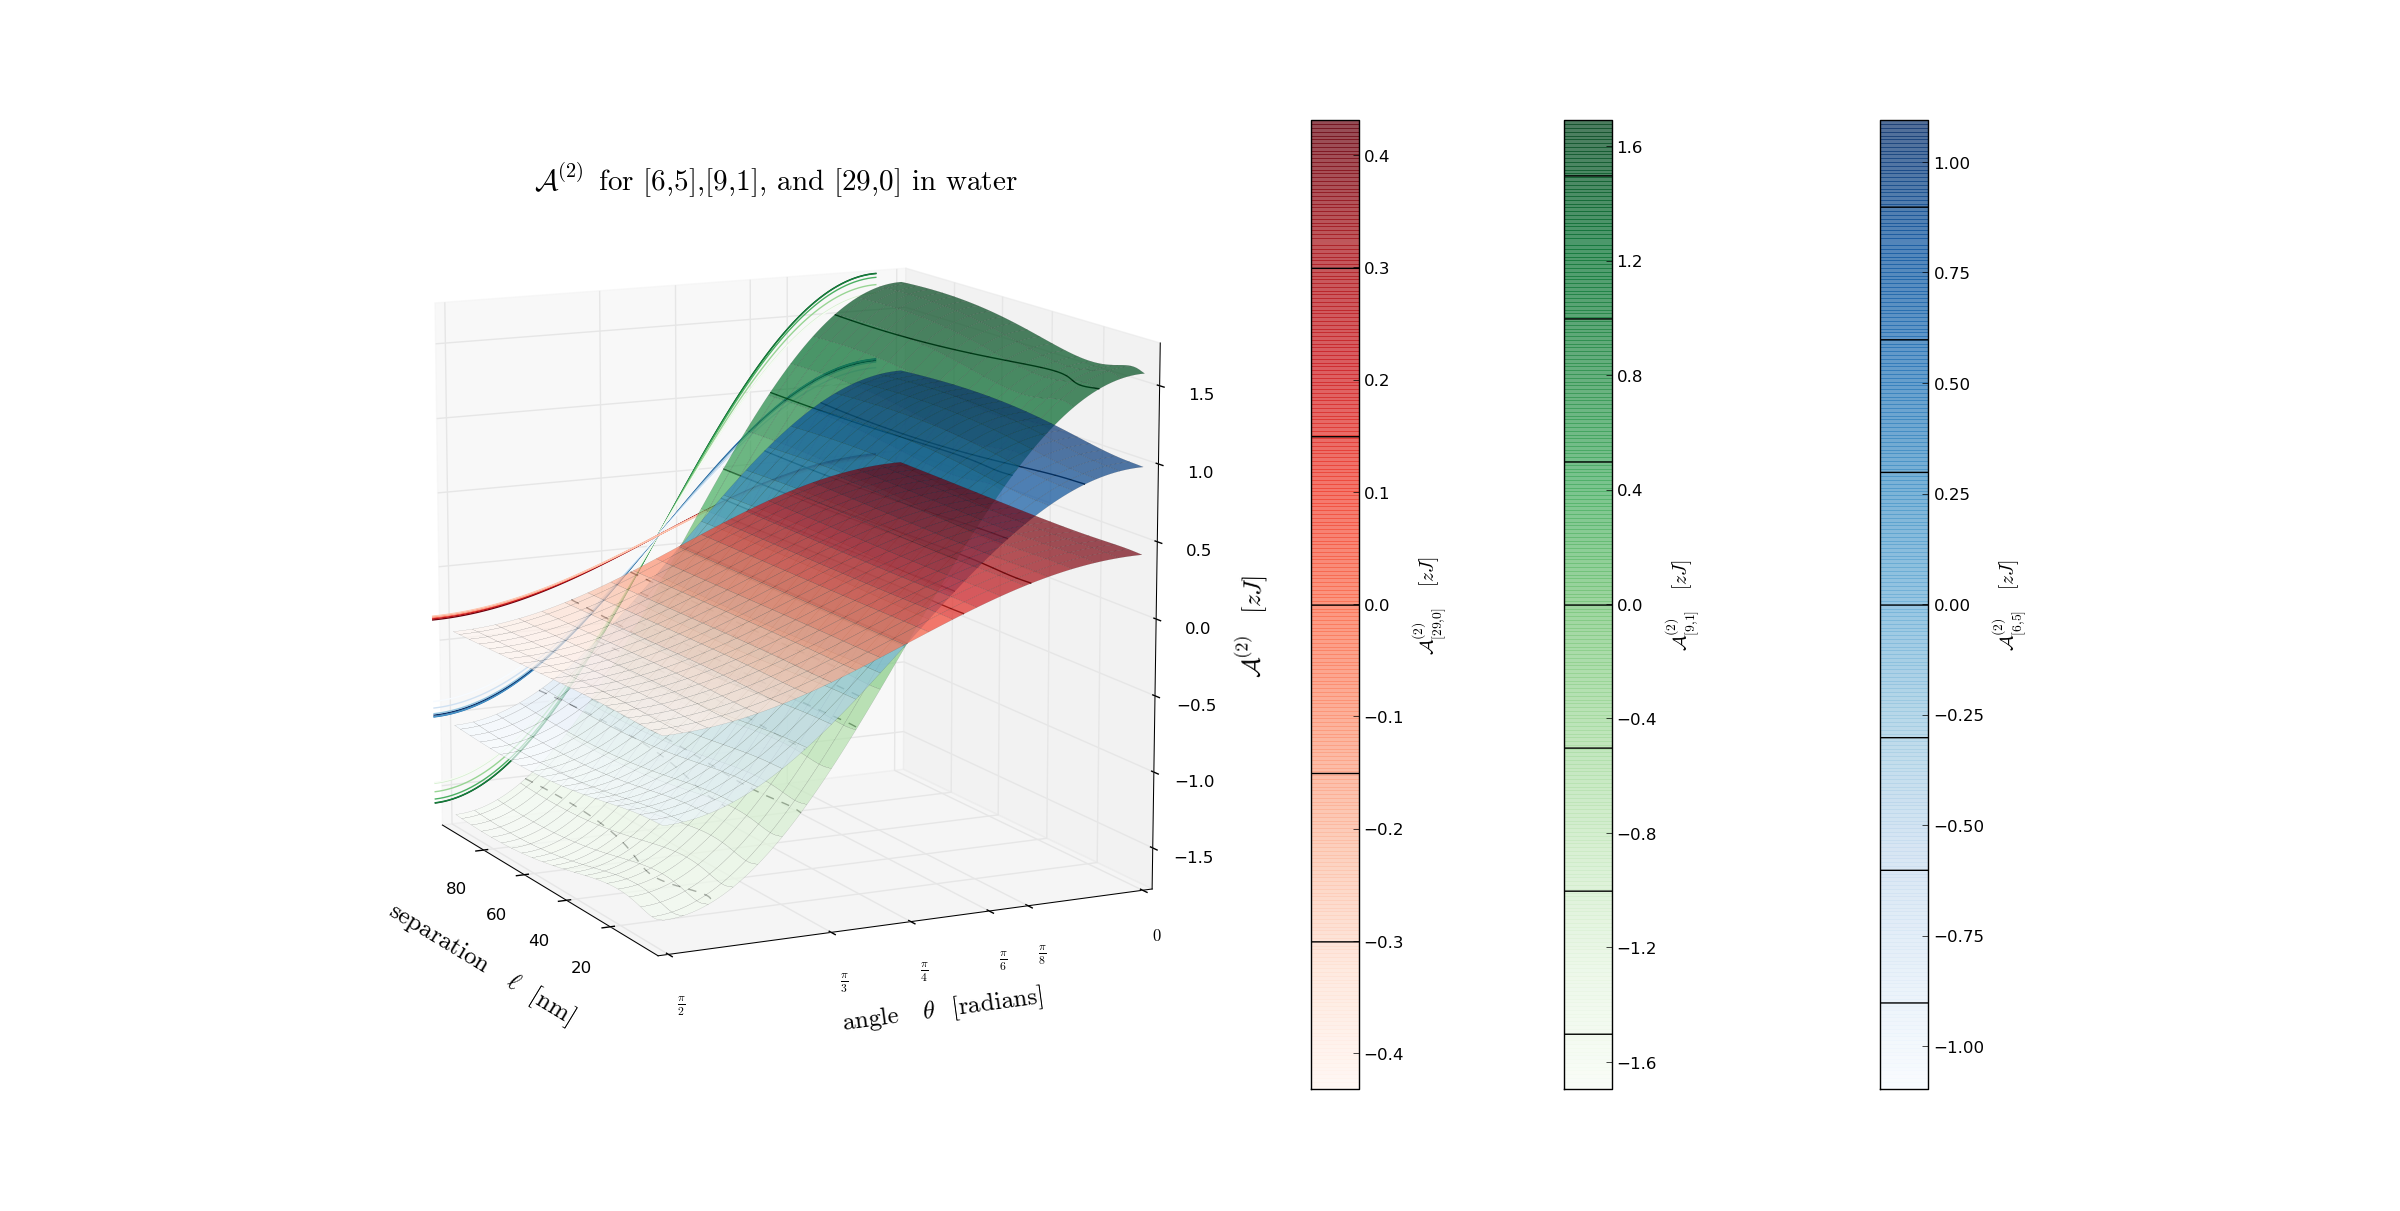
\includegraphics[width=1.5\textwidth]{plots/A2_65_91_290_srw.png}
\hskip 43pt
\caption{$\mathcal{A}^{(2)}$ for [6,5], [9,1], and [29,0] in water.}
\label{eiz65}
\end{center}
\end{figure*} 

\subsection{Total Hamaker: $\mathcal{A} = \mathcal{A}^{(0)}$ + $\mathcal{A}^{(2)}$ for [6,5], [9,1], and [29,0] in water }
%%%%%%%%%A0+A2 COMBO SURF PLOT%%%%%%%%%%%%%%%%%%%%%%%%%%%%%%
\begin{equation}
{\cal A}^{(0)}(\ell) = \frac{k_BT}{32}  {\sum_{n=0}^{\infty}}' \Delta_{1,\parallel} \Delta_{2,\parallel} ~p_n^{4}(\ell) ~\int_0^{\infty} t dt ~\frac{e^{- 2 p_n(\ell) \sqrt{t^{2} + 1}}}{(t^{2} + 1)} \tilde g^{(0)}(t, a_1(i \omega_n), a_2(i \omega_n))
\end{equation}

with

\begin{equation}
\tilde g^{(0)}(t, a_1(i \omega_n), a_2(i \omega_n)) = 2 \left[ (1+3a_1)(1+3a_2) t^{4} + 2 (1+2a_1+2a_2+3a_1a_2) t^{2}  + 2(1+a_1)(1+a_2)\right]
\end{equation}

and

\begin{equation}
{\cal A}^{(2)}(\ell) = \frac{k_BT}{32}  {\sum_{n=0}^{\infty}}' \Delta_{1,\parallel} \Delta_{2,\parallel} ~p_n^{4}(\ell) ~\int_0^{\infty} t dt ~\frac{e^{- 2 p_n(\ell) \sqrt{t^{2} + 1}}}{(t^{2} + 1)} \tilde g^{(2)}(t, a_1(i \omega_n), a_2(i \omega_n), \theta)
\end{equation}

with

\begin{equation}
\tilde g^{(2)}(t, a_1(i \omega_n), a_2(i \omega_n), \theta) = (1-a_1)(1-a_2)(t^{2} + 2)^2
\label{befgqw}
\end{equation}

\begin{figure*}[t!]
\begin{center}
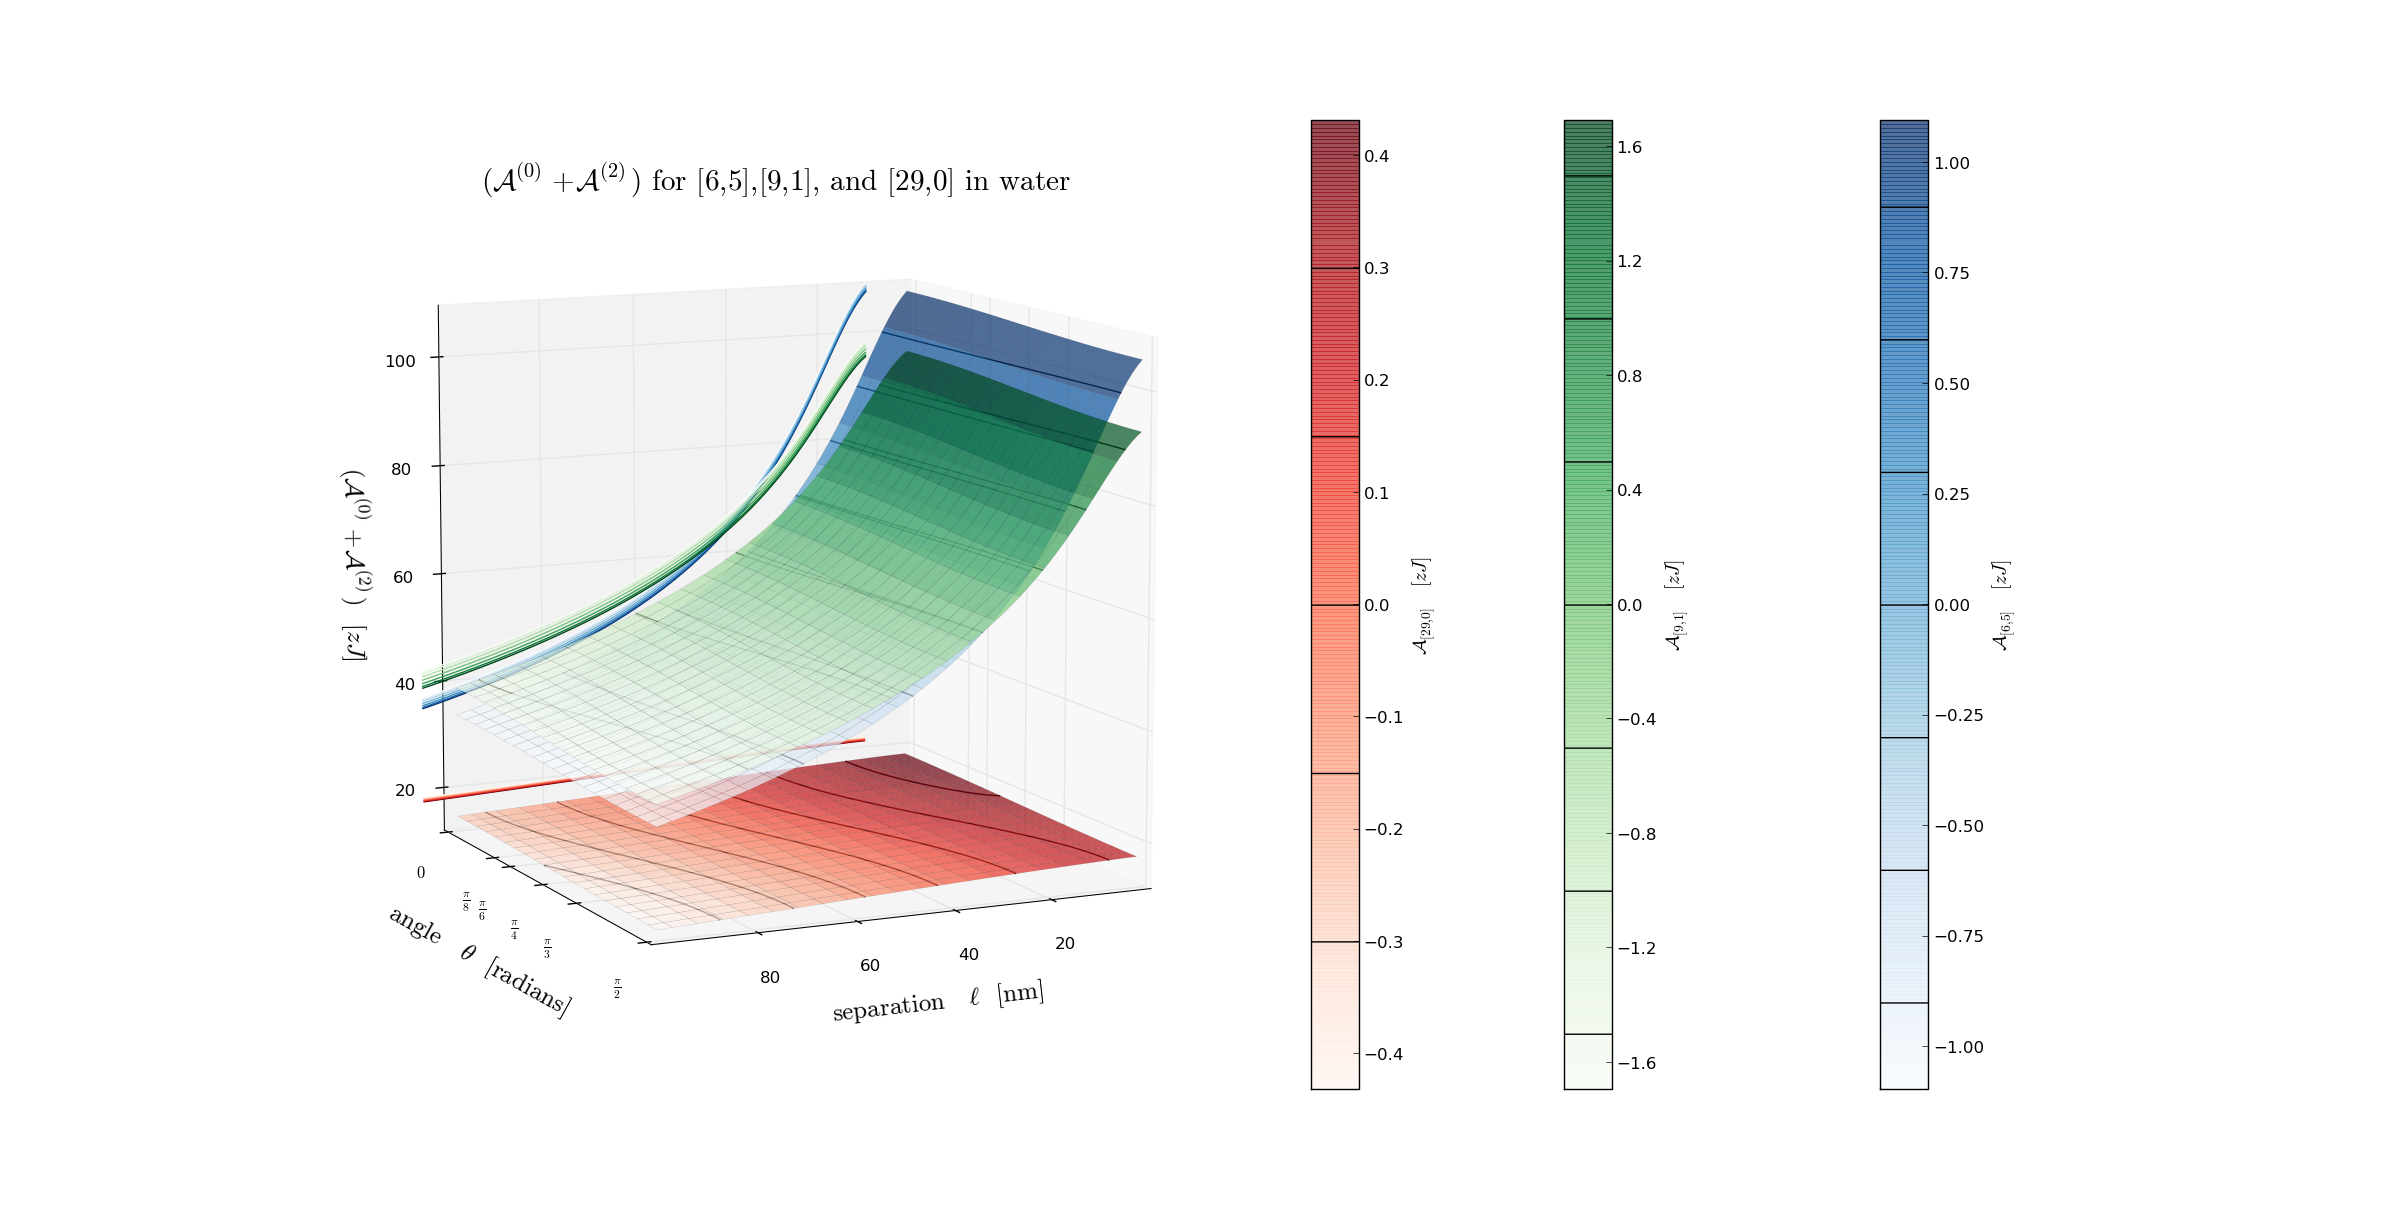
\includegraphics[width=1.5\textwidth]{plots/A_65_91_290_srw.png}
\hskip 43pt
\caption{$\mathcal{A} = \mathcal{A}^{(0)}$ + $\mathcal{A}^{(2)}$ for [6,5], [9,1], and [29,0] in water}
\label{eiz65}
\end{center}
\end{figure*} 

%\section{Non-retarded}
%Here is the second paragraph\footnote{with a footnote}. 
%As you can see it's a rather short paragraph, but not 
%as short as the previous one. This document was 
%created on: \today\ at \currenttime.
%\subsection{A0}
%This is a simple \LaTeX\ document.
%Here is the first paragraph.
%\subsection{A2$\mathcal{A}^{(2)}$ }
%This is a simple \LaTeX\ document.
%Here is the first paragraph.
%\subsection{Atot $\mathcal{A}^{(0)}$ + $\mathcal{A}^{(2)}$ }
%This is a simple \LaTeX\ document.
%Here is the first paragraph.

%%%%%%%%%%%%%%%%%%%%%% TABLES %%%%%%%%%%%%%%%%%%%%%%%%%%%%%%%%%%%%%%%%%%%%%%%%%
\chapter{Tables}
\section{Table of published results}
\begin{table}[ht]
\caption{Rajter results from IJMR perpendiuclar cylinders in water (Rajter's spectrum)}
\centering
\begin{tabular}{l c|c|c}
  \hline  
  &\hspace{0.25in}CNT \hspace{0.25in}& \hspace{0.25in}$\mathcal{A}^{0}$    [zJ] \hspace{0.25in}& \hspace{0.25in}$\mathcal{A}^{2}$    [zJ] \hspace{0.25in}\\
  \hline\hline 
  &[6,5]  & 106 & 1.9 \\
  \hline
  &[9,0]  & \multicolumn{2}{c}{-}\\
  \hline
  &[9,1]  & 92.8 & 3 \\
  \hline
  &[9,3]  & 107 & 36.2 \\
  \hline
  &[29,0] & 18.5 & 0.8 \\
  \hline  
\end{tabular}
\label{table:nonlin}
\end{table}

\section{Table of python results}
\begin{table}[ht]
\caption{Python results, retarded formulation: perpendiuclar cylinders in water, intersurface distance = 1 nm}
\centering
\begin{tabular}{c|c|c|c|c|c|c|c}
  \hline  
  CNT\hspace{0.05in}&atoms*\hspace{0.05in}&radius*[A]\hspace{0.05in}&Type*\hspace{0.05in}&Geom*\hspace{0.05in}&$\mathcal{A}^{0}$(n=0) [zJ]\hspace{0.05in}&$\mathcal{A}^{0}$
  [zJ]\hspace{0.05in}&$\mathcal{A}^{2}$ [zJ]\\
  \hline\hline 
  [6,5]    &364    &3.734      &sc     &chiral     &1x5.46     &105.46    &0.96 \\
  \hline      
  [9,0] &  &   & \multicolumn{2}{c}{semi-metal; in progress}\\
  \hline      
  [9,1]    &364    &3.734      &sc     &chiral     &1x5.46     &93.56      &1.56 \\
  \hline      
  [9,3]    &156    &4.234      &sm     &chiral     &1x5.46     &83.06      &3.23 \\
  \hline      
  [29,0]   &116    &11.352     &sc     &zigzag     &1x5.46     &17.73      &0.41 \\
  \hline  
\end{tabular}
\label{table:nonlin}
\end{table}
*data from 
Chirality-dependent properties of carbon nanotubes: electronic structure, optical dispersion properties, Hamaker coefficients and van der Waals–London dispersion interactions
Rick F. Rajter, Roger H. French, W.Y. Ching, Rudolf Podgornik and V. Adrian Parsegian  
RSC Adv., 2013,3, 823-842
DOI: 10.1039/C2RA20083J

\begin{table}[ht]
\caption{Python results, non-retarded formulation: perpendiuclar cylinders in water}% title of Table
\centering
\begin{tabular}{r c | c | c}
  \hline
  &\hspace{0.25in}CNT\hspace{0.25in}&\hspace{0.25in}$\mathcal{A}^{0}$ [zJ] \hspace{0.25in}& \hspace{0.25in}$\mathcal{A}^{2}$    [zJ] \hspace{0.25in}\\
  \hline\hline                       
  &[6,5]  & 126.80 & 1.16 \\
  \hline
  &[9,0]  & \multicolumn{2}{c}{semi-metal; in progress}\\
  \hline
  &[9,1]  & 112.22 & 1.87 \\
  \hline
  &[9,3]  & \multicolumn{2}{c}{semi-metal; in progress}\\
  \hline
  &[29,0] & 20.93 & 0.49 \\
  \hline  
\end{tabular}
\label{table:nonlin}
\end{table}

\section{Table of Gecko Hamaker results}
\begin{table}[ht]
\caption{Gecko Hamaker results from 2.07, perpendiuclar cylinders in water}
\centering
\begin{tabular}{l c|c|c}
  \hline  
  &\hspace{0.25in}CNT \hspace{0.25in}& \hspace{0.25in}$\mathcal{A}^{0}$    [zJ] \hspace{0.25in}& \hspace{0.25in}$\mathcal{A}^{2}$    [zJ] \hspace{0.25in}\\
  \hline\hline 
  &[6,5]  & 100 & 1.04 \\
  \hline
  &[9,0]  & 151 & 6.96 \\
  \hline
  &[9,1]  & 84.85 & 1.16 \\
  \hline
  &[9,3]  & 80.66 & 1.55 \\
  \hline
  &[29,0] & 17.68 & 0.22 \\
  \hline  
\end{tabular}
\label{table:nonlin}
\end{table}



\end{document}




